\documentclass[twoside]{book}

% Packages required by doxygen
\usepackage{fixltx2e}
\usepackage{calc}
\usepackage{doxygen}
\usepackage[export]{adjustbox} % also loads graphicx
\usepackage{graphicx}
\usepackage[utf8]{inputenc}
\usepackage{makeidx}
\usepackage{multicol}
\usepackage{multirow}
\PassOptionsToPackage{warn}{textcomp}
\usepackage{textcomp}
\usepackage[nointegrals]{wasysym}
\usepackage[table]{xcolor}

% Font selection
\usepackage[T1]{fontenc}
\usepackage[scaled=.90]{helvet}
\usepackage{courier}
\usepackage{amssymb}
\usepackage{sectsty}
\renewcommand{\familydefault}{\sfdefault}
\allsectionsfont{%
  \fontseries{bc}\selectfont%
  \color{darkgray}%
}
\renewcommand{\DoxyLabelFont}{%
  \fontseries{bc}\selectfont%
  \color{darkgray}%
}
\newcommand{\+}{\discretionary{\mbox{\scriptsize$\hookleftarrow$}}{}{}}

% Page & text layout
\usepackage{geometry}
\geometry{%
  a4paper,%
  top=2.5cm,%
  bottom=2.5cm,%
  left=2.5cm,%
  right=2.5cm%
}
\tolerance=750
\hfuzz=15pt
\hbadness=750
\setlength{\emergencystretch}{15pt}
\setlength{\parindent}{0cm}
\setlength{\parskip}{3ex plus 2ex minus 2ex}
\makeatletter
\renewcommand{\paragraph}{%
  \@startsection{paragraph}{4}{0ex}{-1.0ex}{1.0ex}{%
    \normalfont\normalsize\bfseries\SS@parafont%
  }%
}
\renewcommand{\subparagraph}{%
  \@startsection{subparagraph}{5}{0ex}{-1.0ex}{1.0ex}{%
    \normalfont\normalsize\bfseries\SS@subparafont%
  }%
}
\makeatother

% Headers & footers
\usepackage{fancyhdr}
\pagestyle{fancyplain}
\fancyhead[LE]{\fancyplain{}{\bfseries\thepage}}
\fancyhead[CE]{\fancyplain{}{}}
\fancyhead[RE]{\fancyplain{}{\bfseries\leftmark}}
\fancyhead[LO]{\fancyplain{}{\bfseries\rightmark}}
\fancyhead[CO]{\fancyplain{}{}}
\fancyhead[RO]{\fancyplain{}{\bfseries\thepage}}
\fancyfoot[LE]{\fancyplain{}{}}
\fancyfoot[CE]{\fancyplain{}{}}
\fancyfoot[RE]{\fancyplain{}{\bfseries\scriptsize Generated by Doxygen }}
\fancyfoot[LO]{\fancyplain{}{\bfseries\scriptsize Generated by Doxygen }}
\fancyfoot[CO]{\fancyplain{}{}}
\fancyfoot[RO]{\fancyplain{}{}}
\renewcommand{\footrulewidth}{0.4pt}
\renewcommand{\chaptermark}[1]{%
  \markboth{#1}{}%
}
\renewcommand{\sectionmark}[1]{%
  \markright{\thesection\ #1}%
}

% Indices & bibliography
\usepackage{natbib}
\usepackage[titles]{tocloft}
\setcounter{tocdepth}{3}
\setcounter{secnumdepth}{5}
\makeindex

% Hyperlinks (required, but should be loaded last)
\usepackage{ifpdf}
\ifpdf
  \usepackage[pdftex,pagebackref=true]{hyperref}
\else
  \usepackage[ps2pdf,pagebackref=true]{hyperref}
\fi
\hypersetup{%
  colorlinks=true,%
  linkcolor=blue,%
  citecolor=blue,%
  unicode%
}

% Custom commands
\newcommand{\clearemptydoublepage}{%
  \newpage{\pagestyle{empty}\cleardoublepage}%
}

\usepackage{caption}
\captionsetup{labelsep=space,justification=centering,font={bf},singlelinecheck=off,skip=4pt,position=top}

%===== C O N T E N T S =====

\begin{document}

% Titlepage & ToC
\hypersetup{pageanchor=false,
             bookmarksnumbered=true,
             pdfencoding=unicode
            }
\pagenumbering{alph}
\begin{titlepage}
\vspace*{7cm}
\begin{center}%
{\Large Pluri\+Notes }\\
\vspace*{1cm}
{\large Generated by Doxygen 1.8.13}\\
\end{center}
\end{titlepage}
\clearemptydoublepage
\pagenumbering{roman}
\tableofcontents
\clearemptydoublepage
\pagenumbering{arabic}
\hypersetup{pageanchor=true}

%--- Begin generated contents ---
\chapter{Hierarchical Index}
\section{Class Hierarchy}
This inheritance list is sorted roughly, but not completely, alphabetically\+:\begin{DoxyCompactList}
\item \contentsline{section}{Couple}{\pageref{class_couple}}{}
\item \contentsline{section}{Date}{\pageref{class_date}}{}
\item \contentsline{section}{Exception}{\pageref{class_exception}}{}
\item \contentsline{section}{Note}{\pageref{class_note}}{}
\item \contentsline{section}{Notes\+Editor}{\pageref{class_notes_editor}}{}
\item \contentsline{section}{Notes\+Manager}{\pageref{class_notes_manager}}{}
\item \contentsline{section}{Note\+Version}{\pageref{class_note_version}}{}
\begin{DoxyCompactList}
\item \contentsline{section}{Article}{\pageref{class_article}}{}
\item \contentsline{section}{Audio}{\pageref{class_audio}}{}
\item \contentsline{section}{Image}{\pageref{class_image}}{}
\item \contentsline{section}{Task}{\pageref{class_task}}{}
\item \contentsline{section}{Video}{\pageref{class_video}}{}
\end{DoxyCompactList}
\item \contentsline{section}{Note\+Version\+Factory}{\pageref{class_note_version_factory}}{}
\begin{DoxyCompactList}
\item \contentsline{section}{Derived\+Register$<$ T $>$}{\pageref{struct_derived_register}}{}
\item \contentsline{section}{Derived\+Register$<$ Article $>$}{\pageref{struct_derived_register}}{}
\item \contentsline{section}{Derived\+Register$<$ Image $>$}{\pageref{struct_derived_register}}{}
\item \contentsline{section}{Derived\+Register$<$ Task $>$}{\pageref{struct_derived_register}}{}
\end{DoxyCompactList}
\item Q\+Dialog\begin{DoxyCompactList}
\item \contentsline{section}{Trash\+Editor}{\pageref{class_trash_editor}}{}
\end{DoxyCompactList}
\item Q\+Main\+Window\begin{DoxyCompactList}
\item \contentsline{section}{Main\+Window}{\pageref{class_main_window}}{}
\item \contentsline{section}{Main\+Window}{\pageref{class_main_window}}{}
\end{DoxyCompactList}
\item Q\+Widget\begin{DoxyCompactList}
\item \contentsline{section}{Form\+Note}{\pageref{class_form_note}}{}
\item \contentsline{section}{Form\+Version}{\pageref{class_form_version}}{}
\begin{DoxyCompactList}
\item \contentsline{section}{Form\+Article}{\pageref{class_form_article}}{}
\item \contentsline{section}{Form\+Image}{\pageref{class_form_image}}{}
\end{DoxyCompactList}
\item \contentsline{section}{type\+Note}{\pageref{classtype_note}}{}
\end{DoxyCompactList}
\item \contentsline{section}{Relation}{\pageref{class_relation}}{}
\item \contentsline{section}{Relations\+Manager}{\pageref{class_relations_manager}}{}
\item \contentsline{section}{Time\+Exception}{\pageref{class_time_exception}}{}
\item \contentsline{section}{Trash}{\pageref{class_trash}}{}
\end{DoxyCompactList}

\chapter{Class Index}
\section{Class List}
Here are the classes, structs, unions and interfaces with brief descriptions\+:\begin{DoxyCompactList}
\item\contentsline{section}{\hyperlink{class_article}{Article} }{\pageref{class_article}}{}
\item\contentsline{section}{\hyperlink{class_audio}{Audio} }{\pageref{class_audio}}{}
\item\contentsline{section}{\hyperlink{class_couple}{Couple} }{\pageref{class_couple}}{}
\item\contentsline{section}{\hyperlink{class_date}{Date} }{\pageref{class_date}}{}
\item\contentsline{section}{\hyperlink{struct_derived_register}{Derived\+Register$<$ T $>$} }{\pageref{struct_derived_register}}{}
\item\contentsline{section}{\hyperlink{class_exception}{Exception} }{\pageref{class_exception}}{}
\item\contentsline{section}{\hyperlink{class_form_article}{Form\+Article} }{\pageref{class_form_article}}{}
\item\contentsline{section}{\hyperlink{class_form_image}{Form\+Image} }{\pageref{class_form_image}}{}
\item\contentsline{section}{\hyperlink{class_form_note}{Form\+Note} }{\pageref{class_form_note}}{}
\item\contentsline{section}{\hyperlink{class_form_version}{Form\+Version} }{\pageref{class_form_version}}{}
\item\contentsline{section}{\hyperlink{class_image}{Image} }{\pageref{class_image}}{}
\item\contentsline{section}{\hyperlink{class_main_window}{Main\+Window} }{\pageref{class_main_window}}{}
\item\contentsline{section}{\hyperlink{class_note}{Note} }{\pageref{class_note}}{}
\item\contentsline{section}{\hyperlink{class_notes_editor}{Notes\+Editor} }{\pageref{class_notes_editor}}{}
\item\contentsline{section}{\hyperlink{class_notes_manager}{Notes\+Manager} }{\pageref{class_notes_manager}}{}
\item\contentsline{section}{\hyperlink{class_note_version}{Note\+Version} }{\pageref{class_note_version}}{}
\item\contentsline{section}{\hyperlink{class_note_version_factory}{Note\+Version\+Factory} }{\pageref{class_note_version_factory}}{}
\item\contentsline{section}{\hyperlink{class_relation}{Relation} }{\pageref{class_relation}}{}
\item\contentsline{section}{\hyperlink{class_relations_manager}{Relations\+Manager} }{\pageref{class_relations_manager}}{}
\item\contentsline{section}{\hyperlink{class_task}{Task} }{\pageref{class_task}}{}
\item\contentsline{section}{\hyperlink{class_time_exception}{Time\+Exception} }{\pageref{class_time_exception}}{}
\item\contentsline{section}{\hyperlink{class_trash}{Trash} }{\pageref{class_trash}}{}
\item\contentsline{section}{\hyperlink{class_trash_editor}{Trash\+Editor} }{\pageref{class_trash_editor}}{}
\item\contentsline{section}{\hyperlink{classtype_note}{type\+Note} }{\pageref{classtype_note}}{}
\item\contentsline{section}{\hyperlink{class_video}{Video} }{\pageref{class_video}}{}
\end{DoxyCompactList}

\chapter{File Index}
\section{File List}
Here is a list of all documented files with brief descriptions\+:\begin{DoxyCompactList}
\item\contentsline{section}{Documents/\+U\+T\+C/\+G\+I02/\+L\+O21/\+L\+O21/\+Qt\+Version/\hyperlink{date_8h}{date.\+h} \\*Définition du type date }{\pageref{date_8h}}{}
\item\contentsline{section}{Documents/\+U\+T\+C/\+G\+I02/\+L\+O21/\+L\+O21/\+Qt\+Version/{\bfseries Interface\+J.\+h} }{\pageref{_interface_j_8h}}{}
\item\contentsline{section}{Documents/\+U\+T\+C/\+G\+I02/\+L\+O21/\+L\+O21/\+Qt\+Version/{\bfseries mainwindow.\+h} }{\pageref{mainwindow_8h}}{}
\item\contentsline{section}{Documents/\+U\+T\+C/\+G\+I02/\+L\+O21/\+L\+O21/\+Qt\+Version/\hyperlink{note_8h}{note.\+h} \\*Définition de la classe \hyperlink{class_note}{Note} }{\pageref{note_8h}}{}
\item\contentsline{section}{Documents/\+U\+T\+C/\+G\+I02/\+L\+O21/\+L\+O21/\+Qt\+Version/{\bfseries noteseditor.\+h} }{\pageref{noteseditor_8h}}{}
\item\contentsline{section}{Documents/\+U\+T\+C/\+G\+I02/\+L\+O21/\+L\+O21/\+Qt\+Version/\hyperlink{notesmanager_8h}{notesmanager.\+h} \\*Définition de la classe \hyperlink{class_notes_manager}{Notes\+Manager} }{\pageref{notesmanager_8h}}{}
\item\contentsline{section}{Documents/\+U\+T\+C/\+G\+I02/\+L\+O21/\+L\+O21/\+Qt\+Version/\hyperlink{noteversion_8h}{noteversion.\+h} \\*Définition de la classe \hyperlink{class_note_version}{Note\+Version} }{\pageref{noteversion_8h}}{}
\item\contentsline{section}{Documents/\+U\+T\+C/\+G\+I02/\+L\+O21/\+L\+O21/\+Qt\+Version/\hyperlink{plurinotes_8h}{plurinotes.\+h} }{\pageref{plurinotes_8h}}{}
\item\contentsline{section}{Documents/\+U\+T\+C/\+G\+I02/\+L\+O21/\+L\+O21/\+Qt\+Version/\hyperlink{relation_8h}{relation.\+h} \\*Définition de la classe \hyperlink{class_couple}{Couple} et \hyperlink{class_relation}{Relation} }{\pageref{relation_8h}}{}
\item\contentsline{section}{Documents/\+U\+T\+C/\+G\+I02/\+L\+O21/\+L\+O21/\+Qt\+Version/{\bfseries relationsmanager.\+h} }{\pageref{relationsmanager_8h}}{}
\item\contentsline{section}{Documents/\+U\+T\+C/\+G\+I02/\+L\+O21/\+L\+O21/\+Qt\+Version/{\bfseries trash.\+h} }{\pageref{trash_8h}}{}
\item\contentsline{section}{Documents/\+U\+T\+C/\+G\+I02/\+L\+O21/\+L\+O21/\+Qt\+Version/{\bfseries trasheditor.\+h} }{\pageref{trasheditor_8h}}{}
\end{DoxyCompactList}

\chapter{Class Documentation}
\hypertarget{class_article}{}\section{Article Class Reference}
\label{class_article}\index{Article@{Article}}
Inheritance diagram for Article\+:\begin{figure}[H]
\begin{center}
\leavevmode
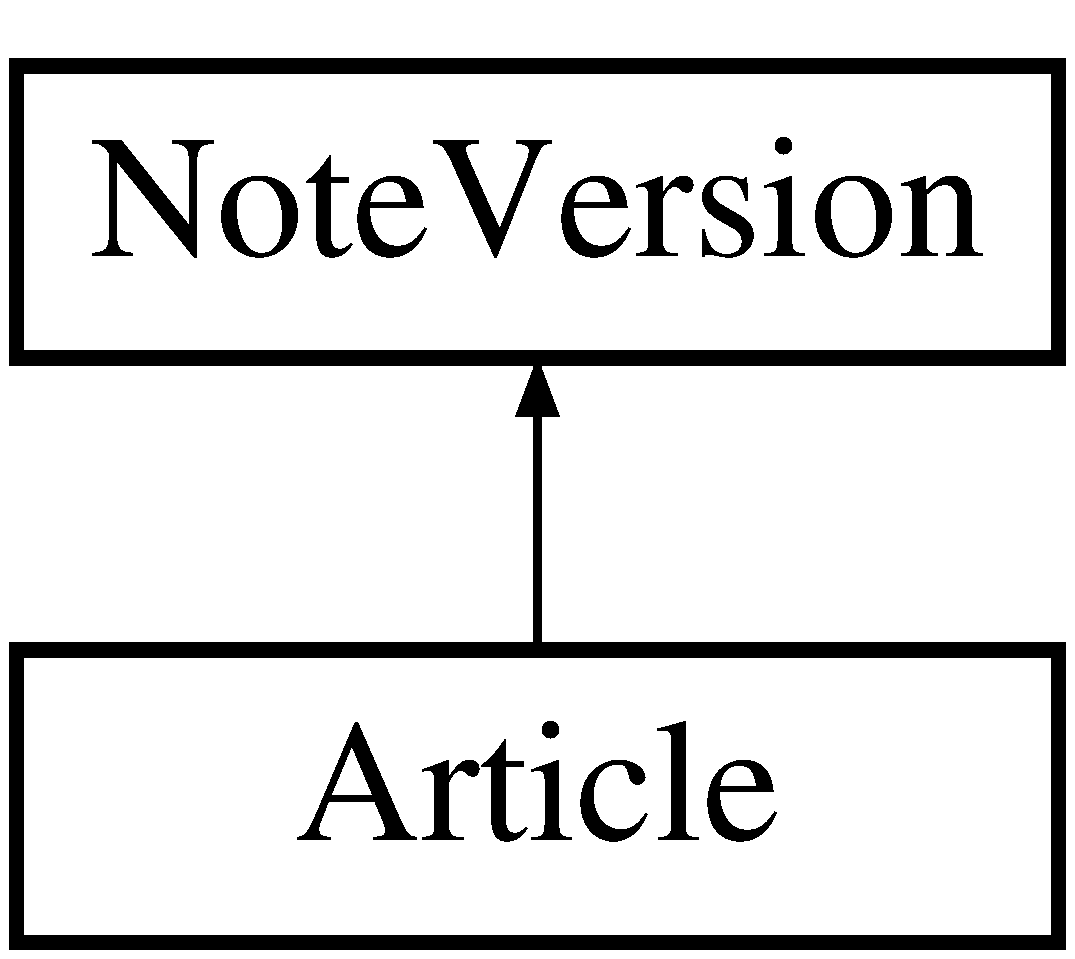
\includegraphics[height=2.000000cm]{class_article}
\end{center}
\end{figure}
\subsection*{Public Member Functions}
\begin{DoxyCompactItemize}
\item 
\hyperlink{class_article_a972ec00d52c495a57f8c657b96280327}{Article} (const Q\+String \&t=Q\+String(), const Q\+String \&te=Q\+String())
\begin{DoxyCompactList}\small\item\em Constructeur de la classe \hyperlink{class_article}{Article}. \end{DoxyCompactList}\item 
\mbox{\Hypertarget{class_article_a66368afb3591b3b4427317e054dd21c7}\label{class_article_a66368afb3591b3b4427317e054dd21c7}} 
const Q\+String \& \hyperlink{class_article_a66368afb3591b3b4427317e054dd21c7}{get\+Text} () const
\begin{DoxyCompactList}\small\item\em accesseur pour obtenir le texte d\textquotesingle{}un article \end{DoxyCompactList}\item 
void \hyperlink{class_article_aaff3219cf9a04413349ff091f1674a26}{set\+Text} (const Q\+String \&str)
\begin{DoxyCompactList}\small\item\em méthode pour appliquer un texte à un article \end{DoxyCompactList}\item 
\hyperlink{class_article}{Article} $\ast$ \hyperlink{class_article_a78188a4d3c5b071caf13db46ecdc32b9}{clone} (unsigned int id) const
\begin{DoxyCompactList}\small\item\em methode clone \end{DoxyCompactList}\item 
\mbox{\Hypertarget{class_article_a85b13c2eb79223ce0c86fa2a82529c60}\label{class_article_a85b13c2eb79223ce0c86fa2a82529c60}} 
Q\+String {\bfseries type} () const
\item 
\mbox{\Hypertarget{class_article_a160945b868825fde17945453e9a70787}\label{class_article_a160945b868825fde17945453e9a70787}} 
\hyperlink{class_form_version}{Form\+Version} $\ast$ {\bfseries form\+Version} ()
\end{DoxyCompactItemize}
\subsection*{Friends}
\begin{DoxyCompactItemize}
\item 
\mbox{\Hypertarget{class_article_a93d7e72623acdfa5b079a11fbf2d9f9d}\label{class_article_a93d7e72623acdfa5b079a11fbf2d9f9d}} 
class {\bfseries Note}
\end{DoxyCompactItemize}
\subsection*{Additional Inherited Members}


\subsection{Constructor \& Destructor Documentation}
\mbox{\Hypertarget{class_article_a972ec00d52c495a57f8c657b96280327}\label{class_article_a972ec00d52c495a57f8c657b96280327}} 
\index{Article@{Article}!Article@{Article}}
\index{Article@{Article}!Article@{Article}}
\subsubsection{\texorpdfstring{Article()}{Article()}}
{\footnotesize\ttfamily Article\+::\+Article (\begin{DoxyParamCaption}\item[{const Q\+String \&}]{t = {\ttfamily QString()},  }\item[{const Q\+String \&}]{te = {\ttfamily QString()} }\end{DoxyParamCaption})}



Constructeur de la classe \hyperlink{class_article}{Article}. 


\begin{DoxyParams}{Parameters}
{\em te} & texte de l\textquotesingle{}article \\
\hline
{\em t} & titre de l\textquotesingle{}article (utilisé par le constructeur de \hyperlink{class_note_version}{Note\+Version}) \\
\hline
\end{DoxyParams}


\subsection{Member Function Documentation}
\mbox{\Hypertarget{class_article_a78188a4d3c5b071caf13db46ecdc32b9}\label{class_article_a78188a4d3c5b071caf13db46ecdc32b9}} 
\index{Article@{Article}!clone@{clone}}
\index{clone@{clone}!Article@{Article}}
\subsubsection{\texorpdfstring{clone()}{clone()}}
{\footnotesize\ttfamily \hyperlink{class_article}{Article} $\ast$ Article\+::clone (\begin{DoxyParamCaption}\item[{unsigned int}]{id }\end{DoxyParamCaption}) const\hspace{0.3cm}{\ttfamily [virtual]}}



methode clone 

\begin{DoxyReturn}{Returns}
un pointeur de \hyperlink{class_article}{Article} sur le clone de l\textquotesingle{}article grâce à l\textquotesingle{}id 
\end{DoxyReturn}

\begin{DoxyParams}{Parameters}
{\em id} & L\textquotesingle{}id de l\textquotesingle{}article que l\textquotesingle{}on souhaite cloner \\
\hline
\end{DoxyParams}


Implements \hyperlink{class_note_version_a7eb23a52291ec623b9bc1b6fe3e86c5a}{Note\+Version}.

\mbox{\Hypertarget{class_article_aaff3219cf9a04413349ff091f1674a26}\label{class_article_aaff3219cf9a04413349ff091f1674a26}} 
\index{Article@{Article}!set\+Text@{set\+Text}}
\index{set\+Text@{set\+Text}!Article@{Article}}
\subsubsection{\texorpdfstring{set\+Text()}{setText()}}
{\footnotesize\ttfamily void Article\+::set\+Text (\begin{DoxyParamCaption}\item[{const Q\+String \&}]{str }\end{DoxyParamCaption})}



méthode pour appliquer un texte à un article 


\begin{DoxyParams}{Parameters}
{\em str} & Texte d\textquotesingle{}une version \\
\hline
\end{DoxyParams}


The documentation for this class was generated from the following files\+:\begin{DoxyCompactItemize}
\item 
Documents/\+G\+I02/\+L\+O21/\+Projet/\+L\+O21/\+Qt\+Version/\hyperlink{noteversion_8h}{noteversion.\+h}\item 
Documents/\+G\+I02/\+L\+O21/\+Projet/\+L\+O21/\+Qt\+Version/noteversion.\+cpp\end{DoxyCompactItemize}

\hypertarget{class_audio}{}\section{Audio Class Reference}
\label{class_audio}\index{Audio@{Audio}}
Inheritance diagram for Audio\+:\begin{figure}[H]
\begin{center}
\leavevmode
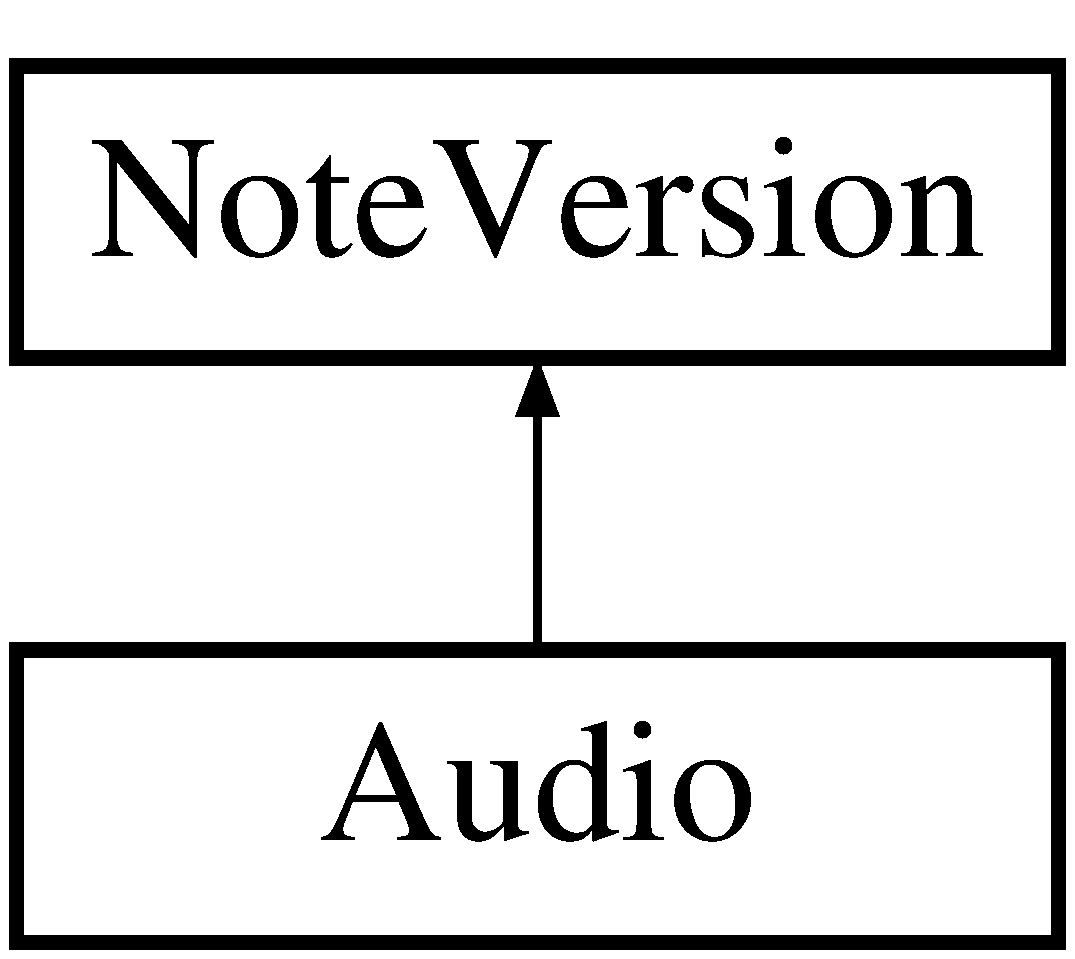
\includegraphics[height=2.000000cm]{class_audio}
\end{center}
\end{figure}
\subsection*{Public Member Functions}
\begin{DoxyCompactItemize}
\item 
\hyperlink{class_audio_aa3944e0eaa26e092079a60585456432a}{Audio} (const Q\+String \&t, const Q\+String \&d, const Q\+String \&f)
\begin{DoxyCompactList}\small\item\em Constructeur de la classe \hyperlink{class_audio}{Audio}. \end{DoxyCompactList}\item 
\mbox{\Hypertarget{class_audio_ad76639dae8c86515da05898e207d86a0}\label{class_audio_ad76639dae8c86515da05898e207d86a0}} 
const Q\+String \& \hyperlink{class_audio_ad76639dae8c86515da05898e207d86a0}{get\+Description} () const
\begin{DoxyCompactList}\small\item\em accesseur pour obtenir la description d\textquotesingle{}une note \hyperlink{class_audio}{Audio} \end{DoxyCompactList}\item 
\mbox{\Hypertarget{class_audio_a1957fb85c894e84902fdabeb160baaa3}\label{class_audio_a1957fb85c894e84902fdabeb160baaa3}} 
const Q\+String \& \hyperlink{class_audio_a1957fb85c894e84902fdabeb160baaa3}{get\+File} () const
\begin{DoxyCompactList}\small\item\em accesseur pour obtenir le fichier d\textquotesingle{}une note \hyperlink{class_audio}{Audio} \end{DoxyCompactList}\item 
\hyperlink{class_audio}{Audio} $\ast$ \hyperlink{class_audio_ae389c3ddd81187769876a1b1790be587}{clone} (unsigned int id) const
\begin{DoxyCompactList}\small\item\em methode clone \end{DoxyCompactList}\item 
\mbox{\Hypertarget{class_audio_a17642cb22e0f2d8d998784497e5f0dca}\label{class_audio_a17642cb22e0f2d8d998784497e5f0dca}} 
Q\+String {\bfseries type} () const
\item 
\mbox{\Hypertarget{class_audio_ae2e6519331aa24cec01988ab2e5fa343}\label{class_audio_ae2e6519331aa24cec01988ab2e5fa343}} 
\hyperlink{class_form_version}{Form\+Version} $\ast$ {\bfseries form\+Version} ()
\end{DoxyCompactItemize}
\subsection*{Friends}
\begin{DoxyCompactItemize}
\item 
\mbox{\Hypertarget{class_audio_a93d7e72623acdfa5b079a11fbf2d9f9d}\label{class_audio_a93d7e72623acdfa5b079a11fbf2d9f9d}} 
class {\bfseries Note}
\end{DoxyCompactItemize}
\subsection*{Additional Inherited Members}


\subsection{Constructor \& Destructor Documentation}
\mbox{\Hypertarget{class_audio_aa3944e0eaa26e092079a60585456432a}\label{class_audio_aa3944e0eaa26e092079a60585456432a}} 
\index{Audio@{Audio}!Audio@{Audio}}
\index{Audio@{Audio}!Audio@{Audio}}
\subsubsection{\texorpdfstring{Audio()}{Audio()}}
{\footnotesize\ttfamily Audio\+::\+Audio (\begin{DoxyParamCaption}\item[{const Q\+String \&}]{t,  }\item[{const Q\+String \&}]{d,  }\item[{const Q\+String \&}]{f }\end{DoxyParamCaption})}



Constructeur de la classe \hyperlink{class_audio}{Audio}. 


\begin{DoxyParams}{Parameters}
{\em t} & titre d\textquotesingle{}une note \hyperlink{class_audio}{Audio} (utilisé par le constructeur de \hyperlink{class_note_version}{Note\+Version}) \\
\hline
{\em d} & description d\textquotesingle{}une note \hyperlink{class_audio}{Audio} \\
\hline
{\em f} & fichier d\textquotesingle{}une note \hyperlink{class_audio}{Audio} \\
\hline
\end{DoxyParams}


\subsection{Member Function Documentation}
\mbox{\Hypertarget{class_audio_ae389c3ddd81187769876a1b1790be587}\label{class_audio_ae389c3ddd81187769876a1b1790be587}} 
\index{Audio@{Audio}!clone@{clone}}
\index{clone@{clone}!Audio@{Audio}}
\subsubsection{\texorpdfstring{clone()}{clone()}}
{\footnotesize\ttfamily \hyperlink{class_audio}{Audio} $\ast$ Audio\+::clone (\begin{DoxyParamCaption}\item[{unsigned int}]{id }\end{DoxyParamCaption}) const\hspace{0.3cm}{\ttfamily [virtual]}}



methode clone 

\begin{DoxyReturn}{Returns}
un pointeur de \hyperlink{class_audio}{Audio} sur le clone de la note \hyperlink{class_audio}{Audio} grâce à l\textquotesingle{}id 
\end{DoxyReturn}

\begin{DoxyParams}{Parameters}
{\em id} & L\textquotesingle{}id de la note \hyperlink{class_audio}{Audio} que l\textquotesingle{}on souhaite cloner \\
\hline
\end{DoxyParams}


Implements \hyperlink{class_note_version_a7eb23a52291ec623b9bc1b6fe3e86c5a}{Note\+Version}.



The documentation for this class was generated from the following files\+:\begin{DoxyCompactItemize}
\item 
Documents/\+U\+T\+C/\+G\+I02/\+L\+O21/\+L\+O21/\+Qt\+Version/\hyperlink{noteversion_8h}{noteversion.\+h}\item 
Documents/\+U\+T\+C/\+G\+I02/\+L\+O21/\+L\+O21/\+Qt\+Version/noteversion.\+cpp\end{DoxyCompactItemize}

\hypertarget{class_couple}{}\section{Couple Class Reference}
\label{class_couple}\index{Couple@{Couple}}
\subsection*{Public Member Functions}
\begin{DoxyCompactItemize}
\item 
\mbox{\Hypertarget{class_couple_a0000c961b867947f39e76a6f0ea04527}\label{class_couple_a0000c961b867947f39e76a6f0ea04527}} 
{\bfseries Couple} (\hyperlink{class_note}{Note} \&id1, \hyperlink{class_note}{Note} \&id2, const Q\+String \&l=\char`\"{}\char`\"{})
\item 
\mbox{\Hypertarget{class_couple_ab1e111ccd47d953bce5a485a40f6e7d2}\label{class_couple_ab1e111ccd47d953bce5a485a40f6e7d2}} 
const \hyperlink{class_note}{Note} \& {\bfseries get\+Note1} () const
\item 
\mbox{\Hypertarget{class_couple_ad3d28199ad0170f65c4564a910167ed6}\label{class_couple_ad3d28199ad0170f65c4564a910167ed6}} 
const \hyperlink{class_note}{Note} \& {\bfseries get\+Note2} () const
\end{DoxyCompactItemize}


The documentation for this class was generated from the following file\+:\begin{DoxyCompactItemize}
\item 
Documents/\+U\+T\+C/\+G\+I02/\+L\+O21/\+L\+O21/\+Qt\+Version/\hyperlink{relation_8h}{relation.\+h}\end{DoxyCompactItemize}

\hypertarget{class_date}{}\section{Date Class Reference}
\label{class_date}\index{Date@{Date}}
\subsection*{Public Member Functions}
\begin{DoxyCompactItemize}
\item 
\hyperlink{class_date_afbee955665b0aeb1a62764c0984628ca}{Date} (unsigned int short j=1, unsigned int short m=1, unsigned int a=0)
\begin{DoxyCompactList}\small\item\em Constructeur à partir d\textquotesingle{}un jour, mois, année. \end{DoxyCompactList}\item 
unsigned short int \hyperlink{class_date_af62b5126cdc9296302151791b333c8c5}{get\+Jour} () const
\begin{DoxyCompactList}\small\item\em Retourne le jour de la date. \end{DoxyCompactList}\item 
unsigned short int \hyperlink{class_date_a42e4cba117fe2bf546509313cba561c8}{get\+Mois} () const
\begin{DoxyCompactList}\small\item\em Retourne le mois de la date. \end{DoxyCompactList}\item 
unsigned int \hyperlink{class_date_aa0da782e7848c098e8bff1b6ecbf6880}{get\+Annee} () const
\begin{DoxyCompactList}\small\item\em Retourne l\textquotesingle{}année de la date. \end{DoxyCompactList}\item 
void \hyperlink{class_date_a7419902750e61b9473ab05ccd5ced33d}{set\+Date} (unsigned short int j, unsigned short int m, unsigned int a)
\begin{DoxyCompactList}\small\item\em initialisation de la date \end{DoxyCompactList}\item 
void \hyperlink{class_date_aa1d8af4081975eb4a323afd962a25fd7}{afficher} (std\+::ostream \&f=std\+::cout) const
\begin{DoxyCompactList}\small\item\em affiche le date sous le format J\+J/\+M\+M/\+A\+A\+AA \end{DoxyCompactList}\item 
bool \hyperlink{class_date_a16b90fa191e5d3080aa558fb29c676d2}{operator==} (const \hyperlink{class_date}{Date} \&d) const
\begin{DoxyCompactList}\small\item\em d1==d2 retourne vrai si les deux dates sont égales \end{DoxyCompactList}\item 
bool \hyperlink{class_date_a42bf31e1ff4d0cfcf71849876e670a1b}{operator$<$} (const \hyperlink{class_date}{Date} \&d) const
\begin{DoxyCompactList}\small\item\em Compare deux dates dans le temps. \end{DoxyCompactList}\item 
int \hyperlink{class_date_adcce792d461f182f9f3107e98029f8a8}{operator-\/} (const \hyperlink{class_date}{Date} \&d) const
\begin{DoxyCompactList}\small\item\em Retourne le nombre de jours séparant les deux dates. \end{DoxyCompactList}\item 
void \hyperlink{class_date_a4a148f744c00b74fff4ead1bed014d64}{today} ()
\begin{DoxyCompactList}\small\item\em Met à jour la date appelant cette méthode avec la date du jour. \end{DoxyCompactList}\item 
\hyperlink{class_date}{Date} \hyperlink{class_date_abed6f57b6368b738e37b6ad9a4c99879}{demain} () const
\begin{DoxyCompactList}\small\item\em Retourne la date du lendemain. \end{DoxyCompactList}\item 
\hyperlink{class_date}{Date} \hyperlink{class_date_ad5cfa3a4ad369bcbc59c0fbacd775fc5}{operator+} (unsigned int nb) const
\begin{DoxyCompactList}\small\item\em Retourne la date dans nb jours. \end{DoxyCompactList}\end{DoxyCompactItemize}


\subsection{Constructor \& Destructor Documentation}
\mbox{\Hypertarget{class_date_afbee955665b0aeb1a62764c0984628ca}\label{class_date_afbee955665b0aeb1a62764c0984628ca}} 
\index{Date@{Date}!Date@{Date}}
\index{Date@{Date}!Date@{Date}}
\subsubsection{\texorpdfstring{Date()}{Date()}}
{\footnotesize\ttfamily Date\+::\+Date (\begin{DoxyParamCaption}\item[{unsigned int short}]{j = {\ttfamily 1},  }\item[{unsigned int short}]{m = {\ttfamily 1},  }\item[{unsigned int}]{a = {\ttfamily 0} }\end{DoxyParamCaption})\hspace{0.3cm}{\ttfamily [inline]}}



Constructeur à partir d\textquotesingle{}un jour, mois, année. 


\begin{DoxyParams}{Parameters}
{\em j} & jour avec 1$<$=j$<$=31 \\
\hline
{\em m} & mois avec 1$<$=m$<$=12 \\
\hline
{\em a} & année avec a$>$=0 \\
\hline
\end{DoxyParams}


\subsection{Member Function Documentation}
\mbox{\Hypertarget{class_date_aa1d8af4081975eb4a323afd962a25fd7}\label{class_date_aa1d8af4081975eb4a323afd962a25fd7}} 
\index{Date@{Date}!afficher@{afficher}}
\index{afficher@{afficher}!Date@{Date}}
\subsubsection{\texorpdfstring{afficher()}{afficher()}}
{\footnotesize\ttfamily void Date\+::afficher (\begin{DoxyParamCaption}\item[{std\+::ostream \&}]{f = {\ttfamily std\+:\+:cout} }\end{DoxyParamCaption}) const}



affiche le date sous le format J\+J/\+M\+M/\+A\+A\+AA 


\begin{DoxyParams}{Parameters}
{\em f} & flux de sortie \\
\hline
\end{DoxyParams}
\mbox{\Hypertarget{class_date_abed6f57b6368b738e37b6ad9a4c99879}\label{class_date_abed6f57b6368b738e37b6ad9a4c99879}} 
\index{Date@{Date}!demain@{demain}}
\index{demain@{demain}!Date@{Date}}
\subsubsection{\texorpdfstring{demain()}{demain()}}
{\footnotesize\ttfamily \hyperlink{class_date}{Date} Date\+::demain (\begin{DoxyParamCaption}{ }\end{DoxyParamCaption}) const}



Retourne la date du lendemain. 

Donne la date du lendemain où la méthodes est appelée \mbox{\Hypertarget{class_date_aa0da782e7848c098e8bff1b6ecbf6880}\label{class_date_aa0da782e7848c098e8bff1b6ecbf6880}} 
\index{Date@{Date}!get\+Annee@{get\+Annee}}
\index{get\+Annee@{get\+Annee}!Date@{Date}}
\subsubsection{\texorpdfstring{get\+Annee()}{getAnnee()}}
{\footnotesize\ttfamily unsigned int Date\+::get\+Annee (\begin{DoxyParamCaption}{ }\end{DoxyParamCaption}) const\hspace{0.3cm}{\ttfamily [inline]}}



Retourne l\textquotesingle{}année de la date. 


\begin{DoxyParams}{Parameters}
{\em annee} & $>$=0 \\
\hline
\end{DoxyParams}
\mbox{\Hypertarget{class_date_af62b5126cdc9296302151791b333c8c5}\label{class_date_af62b5126cdc9296302151791b333c8c5}} 
\index{Date@{Date}!get\+Jour@{get\+Jour}}
\index{get\+Jour@{get\+Jour}!Date@{Date}}
\subsubsection{\texorpdfstring{get\+Jour()}{getJour()}}
{\footnotesize\ttfamily unsigned short int Date\+::get\+Jour (\begin{DoxyParamCaption}{ }\end{DoxyParamCaption}) const\hspace{0.3cm}{\ttfamily [inline]}}



Retourne le jour de la date. 


\begin{DoxyParams}{Parameters}
{\em 1} & $<$= jour $<$= 31 \\
\hline
\end{DoxyParams}
\mbox{\Hypertarget{class_date_a42e4cba117fe2bf546509313cba561c8}\label{class_date_a42e4cba117fe2bf546509313cba561c8}} 
\index{Date@{Date}!get\+Mois@{get\+Mois}}
\index{get\+Mois@{get\+Mois}!Date@{Date}}
\subsubsection{\texorpdfstring{get\+Mois()}{getMois()}}
{\footnotesize\ttfamily unsigned short int Date\+::get\+Mois (\begin{DoxyParamCaption}{ }\end{DoxyParamCaption}) const\hspace{0.3cm}{\ttfamily [inline]}}



Retourne le mois de la date. 


\begin{DoxyParams}{Parameters}
{\em 1} & $<$= mois $<$= 12 \\
\hline
\end{DoxyParams}
\mbox{\Hypertarget{class_date_ad5cfa3a4ad369bcbc59c0fbacd775fc5}\label{class_date_ad5cfa3a4ad369bcbc59c0fbacd775fc5}} 
\index{Date@{Date}!operator+@{operator+}}
\index{operator+@{operator+}!Date@{Date}}
\subsubsection{\texorpdfstring{operator+()}{operator+()}}
{\footnotesize\ttfamily \hyperlink{class_date}{Date} Date\+::operator+ (\begin{DoxyParamCaption}\item[{unsigned int}]{nb }\end{DoxyParamCaption}) const}



Retourne la date dans nb jours. 


\begin{DoxyParams}{Parameters}
{\em nb} & nombre de jours\\
\hline
\end{DoxyParams}
Donne la date actuelle à laquelle on ajoute nb jours. En respectant bien entendu le format d\textquotesingle{}une date. \mbox{\Hypertarget{class_date_adcce792d461f182f9f3107e98029f8a8}\label{class_date_adcce792d461f182f9f3107e98029f8a8}} 
\index{Date@{Date}!operator-\/@{operator-\/}}
\index{operator-\/@{operator-\/}!Date@{Date}}
\subsubsection{\texorpdfstring{operator-\/()}{operator-()}}
{\footnotesize\ttfamily int Date\+::operator-\/ (\begin{DoxyParamCaption}\item[{const \hyperlink{class_date}{Date} \&}]{d }\end{DoxyParamCaption}) const}



Retourne le nombre de jours séparant les deux dates. 


\begin{DoxyParams}{Parameters}
{\em d} & date \\
\hline
\end{DoxyParams}
\mbox{\Hypertarget{class_date_a42bf31e1ff4d0cfcf71849876e670a1b}\label{class_date_a42bf31e1ff4d0cfcf71849876e670a1b}} 
\index{Date@{Date}!operator$<$@{operator$<$}}
\index{operator$<$@{operator$<$}!Date@{Date}}
\subsubsection{\texorpdfstring{operator$<$()}{operator<()}}
{\footnotesize\ttfamily bool Date\+::operator$<$ (\begin{DoxyParamCaption}\item[{const \hyperlink{class_date}{Date} \&}]{d }\end{DoxyParamCaption}) const}



Compare deux dates dans le temps. 


\begin{DoxyParams}{Parameters}
{\em d} & date\\
\hline
\end{DoxyParams}
d1$<$d2 retourne true si d1 est avant d2 \mbox{\Hypertarget{class_date_a16b90fa191e5d3080aa558fb29c676d2}\label{class_date_a16b90fa191e5d3080aa558fb29c676d2}} 
\index{Date@{Date}!operator==@{operator==}}
\index{operator==@{operator==}!Date@{Date}}
\subsubsection{\texorpdfstring{operator==()}{operator==()}}
{\footnotesize\ttfamily bool Date\+::operator== (\begin{DoxyParamCaption}\item[{const \hyperlink{class_date}{Date} \&}]{d }\end{DoxyParamCaption}) const}



d1==d2 retourne vrai si les deux dates sont égales 


\begin{DoxyParams}{Parameters}
{\em d} & date\\
\hline
\end{DoxyParams}
on va comparer la date d avec la date appelant la méthode pour voir si elles sont égales \mbox{\Hypertarget{class_date_a7419902750e61b9473ab05ccd5ced33d}\label{class_date_a7419902750e61b9473ab05ccd5ced33d}} 
\index{Date@{Date}!set\+Date@{set\+Date}}
\index{set\+Date@{set\+Date}!Date@{Date}}
\subsubsection{\texorpdfstring{set\+Date()}{setDate()}}
{\footnotesize\ttfamily void Date\+::set\+Date (\begin{DoxyParamCaption}\item[{unsigned short int}]{j,  }\item[{unsigned short int}]{m,  }\item[{unsigned int}]{a }\end{DoxyParamCaption})}



initialisation de la date 


\begin{DoxyParams}{Parameters}
{\em j} & jour avec 1$<$=j$<$=31 \\
\hline
{\em m} & mois avec 1$<$=m$<$=12 \\
\hline
{\em a} & année avec a$>$=0 \\
\hline
\end{DoxyParams}
\mbox{\Hypertarget{class_date_a4a148f744c00b74fff4ead1bed014d64}\label{class_date_a4a148f744c00b74fff4ead1bed014d64}} 
\index{Date@{Date}!today@{today}}
\index{today@{today}!Date@{Date}}
\subsubsection{\texorpdfstring{today()}{today()}}
{\footnotesize\ttfamily void Date\+::today (\begin{DoxyParamCaption}{ }\end{DoxyParamCaption})}



Met à jour la date appelant cette méthode avec la date du jour. 

Donne la date du jour même où la méthodes est appelée 

The documentation for this class was generated from the following files\+:\begin{DoxyCompactItemize}
\item 
Documents/\+G\+I02/\+L\+O21/\+Projet/\+L\+O21/\+Qt\+Version/\hyperlink{date_8h}{date.\+h}\item 
Documents/\+G\+I02/\+L\+O21/\+Projet/\+L\+O21/\+Qt\+Version/date.\+cpp\end{DoxyCompactItemize}

\hypertarget{struct_derived_register}{}\section{Derived\+Register$<$ T $>$ Struct Template Reference}
\label{struct_derived_register}\index{Derived\+Register$<$ T $>$@{Derived\+Register$<$ T $>$}}
Inheritance diagram for Derived\+Register$<$ T $>$\+:\begin{figure}[H]
\begin{center}
\leavevmode
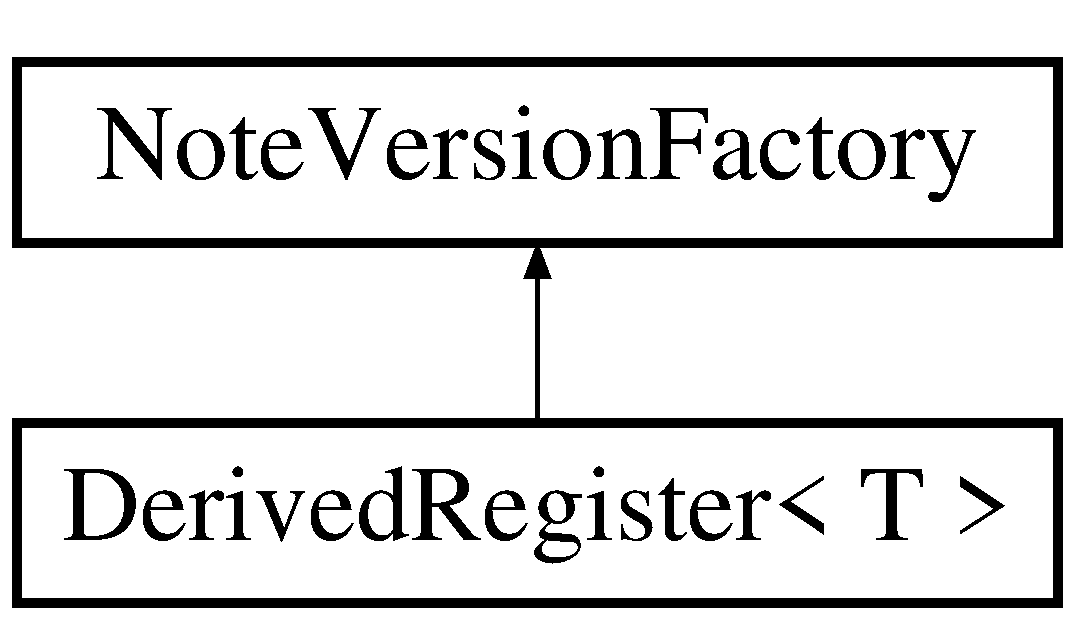
\includegraphics[height=2.000000cm]{struct_derived_register}
\end{center}
\end{figure}
\subsection*{Public Member Functions}
\begin{DoxyCompactItemize}
\item 
\mbox{\Hypertarget{struct_derived_register_af89892a9b8487f33b8824b662d2a6f4a}\label{struct_derived_register_af89892a9b8487f33b8824b662d2a6f4a}} 
{\bfseries Derived\+Register} (Q\+String const \&s)
\end{DoxyCompactItemize}
\subsection*{Additional Inherited Members}


The documentation for this struct was generated from the following file\+:\begin{DoxyCompactItemize}
\item 
Documents/\+U\+T\+C/\+G\+I02/\+L\+O21/\+L\+O21/\+Qt\+Version/\hyperlink{noteversion_8h}{noteversion.\+h}\end{DoxyCompactItemize}

\hypertarget{class_exception}{}\section{Exception Class Reference}
\label{class_exception}\index{Exception@{Exception}}
\subsection*{Public Member Functions}
\begin{DoxyCompactItemize}
\item 
\mbox{\Hypertarget{class_exception_a72d06f00500f1b551adadd188a1e1f33}\label{class_exception_a72d06f00500f1b551adadd188a1e1f33}} 
{\bfseries Exception} (const Q\+String \&str)
\item 
\mbox{\Hypertarget{class_exception_a378568dd6f6421f43d323db53c2e5fe7}\label{class_exception_a378568dd6f6421f43d323db53c2e5fe7}} 
const Q\+String \& {\bfseries get\+Info} () const
\end{DoxyCompactItemize}


The documentation for this class was generated from the following file\+:\begin{DoxyCompactItemize}
\item 
Documents/\+U\+T\+C/\+G\+I02/\+L\+O21/\+L\+O21/\+Qt\+Version/\hyperlink{note_8h}{note.\+h}\end{DoxyCompactItemize}

\hypertarget{class_form_article}{}\section{Form\+Article Class Reference}
\label{class_form_article}\index{Form\+Article@{Form\+Article}}
Inheritance diagram for Form\+Article\+:\begin{figure}[H]
\begin{center}
\leavevmode
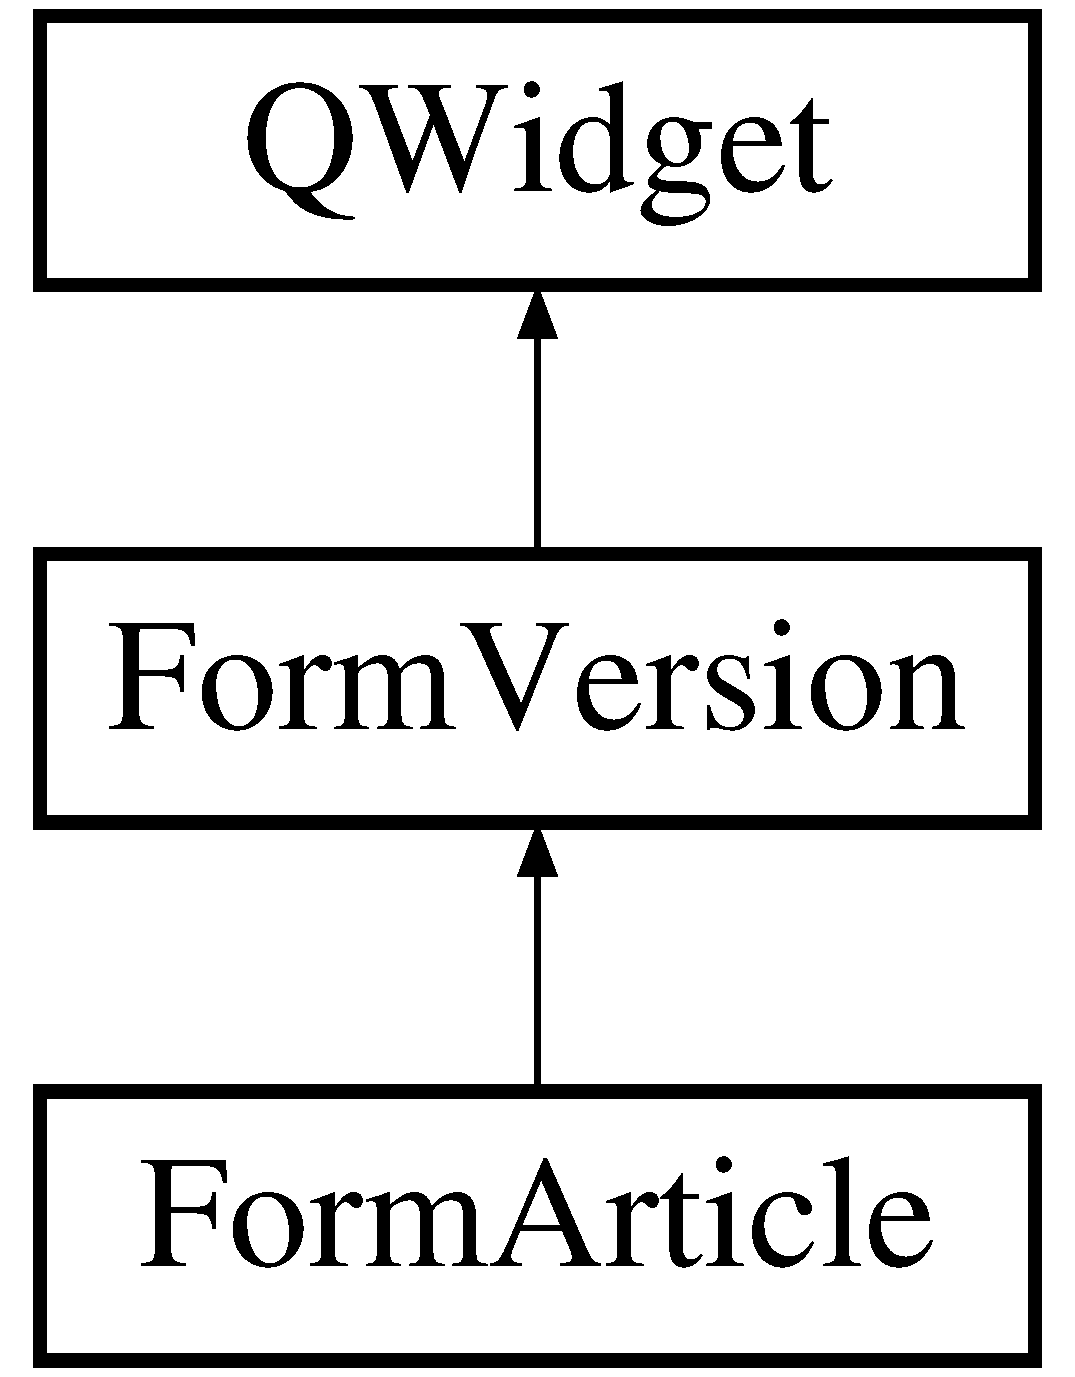
\includegraphics[height=3.000000cm]{class_form_article}
\end{center}
\end{figure}
\subsection*{Public Member Functions}
\begin{DoxyCompactItemize}
\item 
\mbox{\Hypertarget{class_form_article_a751d2c68185be1aff70c66121626b1c8}\label{class_form_article_a751d2c68185be1aff70c66121626b1c8}} 
{\bfseries Form\+Article} (\hyperlink{class_article}{Article} $\ast$a, Q\+Widget $\ast$parent=0)
\item 
\mbox{\Hypertarget{class_form_article_a88488a9f4a72015f6e2bc410e086ebe5}\label{class_form_article_a88488a9f4a72015f6e2bc410e086ebe5}} 
void {\bfseries save\+Version} (\hyperlink{class_note_version}{Note\+Version} $\ast$ver)
\end{DoxyCompactItemize}


The documentation for this class was generated from the following files\+:\begin{DoxyCompactItemize}
\item 
Documents/\+G\+I02/\+L\+O21/\+Projet/\+L\+O21/\+Qt\+Version/\hyperlink{noteversion_8h}{noteversion.\+h}\item 
Documents/\+G\+I02/\+L\+O21/\+Projet/\+L\+O21/\+Qt\+Version/noteversion.\+cpp\end{DoxyCompactItemize}

\hypertarget{class_form_image}{}\section{Form\+Image Class Reference}
\label{class_form_image}\index{Form\+Image@{Form\+Image}}
Inheritance diagram for Form\+Image\+:\begin{figure}[H]
\begin{center}
\leavevmode
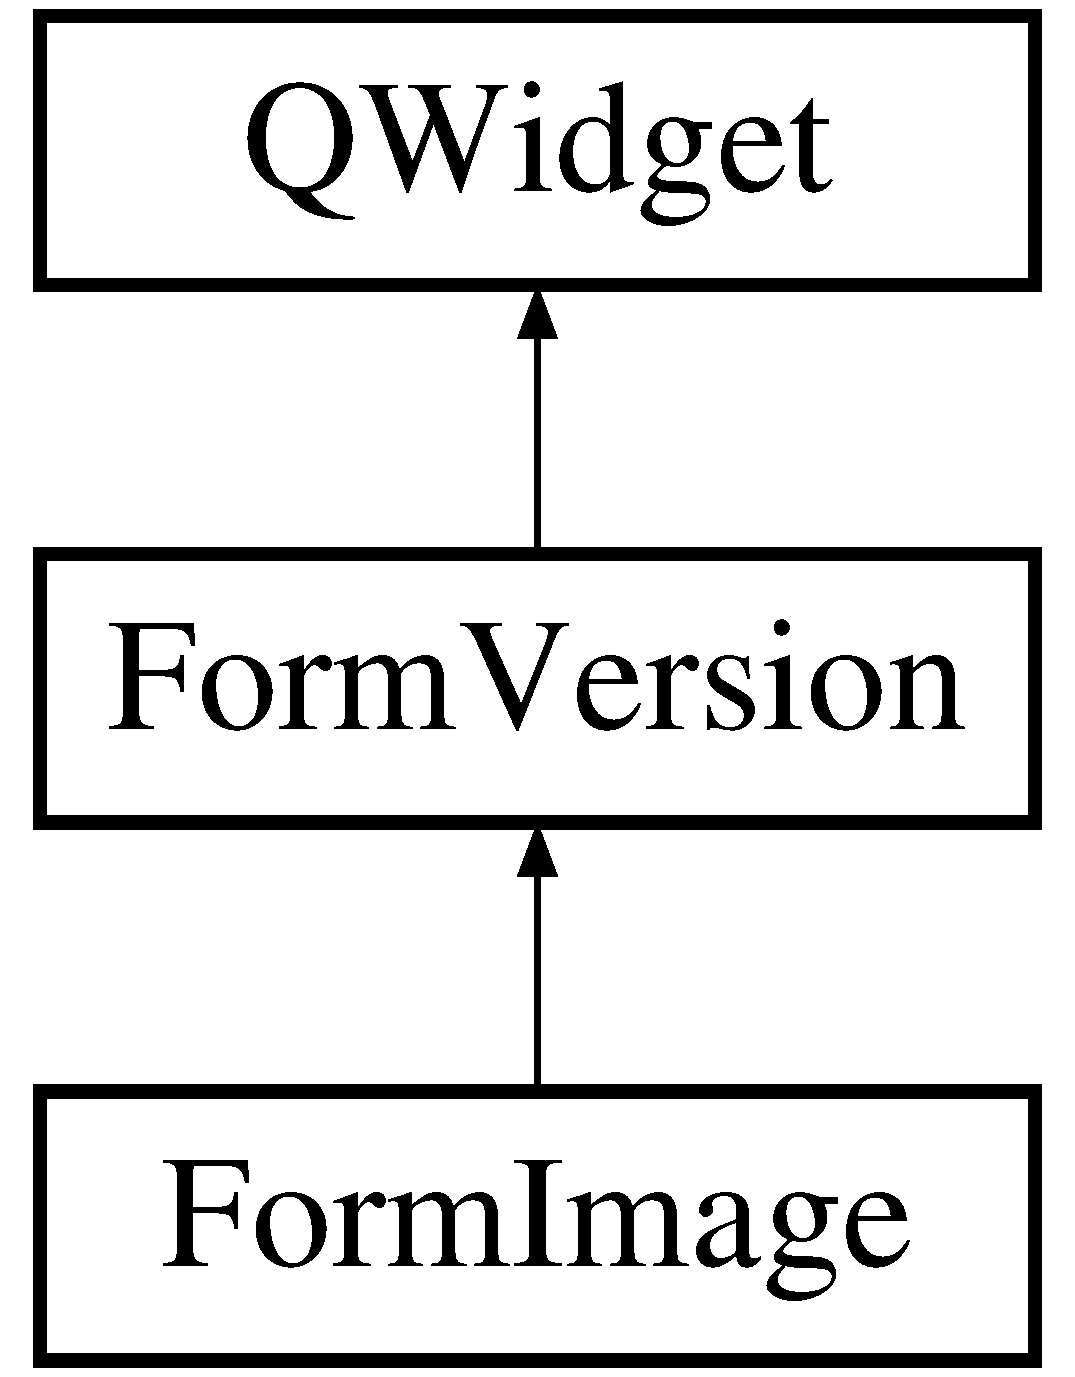
\includegraphics[height=3.000000cm]{class_form_image}
\end{center}
\end{figure}
\subsection*{Public Member Functions}
\begin{DoxyCompactItemize}
\item 
\mbox{\Hypertarget{class_form_image_aea7e0896a70f60a08fedc80a87cb6534}\label{class_form_image_aea7e0896a70f60a08fedc80a87cb6534}} 
{\bfseries Form\+Image} (\hyperlink{class_image}{Image} $\ast$a, Q\+Widget $\ast$parent=0)
\item 
\mbox{\Hypertarget{class_form_image_a3fb6e3870e4c2217c9c7a58fe67072d3}\label{class_form_image_a3fb6e3870e4c2217c9c7a58fe67072d3}} 
void {\bfseries save\+Version} (\hyperlink{class_note_version}{Note\+Version} $\ast$)
\end{DoxyCompactItemize}


The documentation for this class was generated from the following files\+:\begin{DoxyCompactItemize}
\item 
Documents/\+U\+T\+C/\+G\+I02/\+L\+O21/\+L\+O21/\+Qt\+Version/\hyperlink{noteversion_8h}{noteversion.\+h}\item 
Documents/\+U\+T\+C/\+G\+I02/\+L\+O21/\+L\+O21/\+Qt\+Version/noteversion.\+cpp\end{DoxyCompactItemize}

\hypertarget{class_form_note}{}\section{Form\+Note Class Reference}
\label{class_form_note}\index{Form\+Note@{Form\+Note}}
Inheritance diagram for Form\+Note\+:\begin{figure}[H]
\begin{center}
\leavevmode
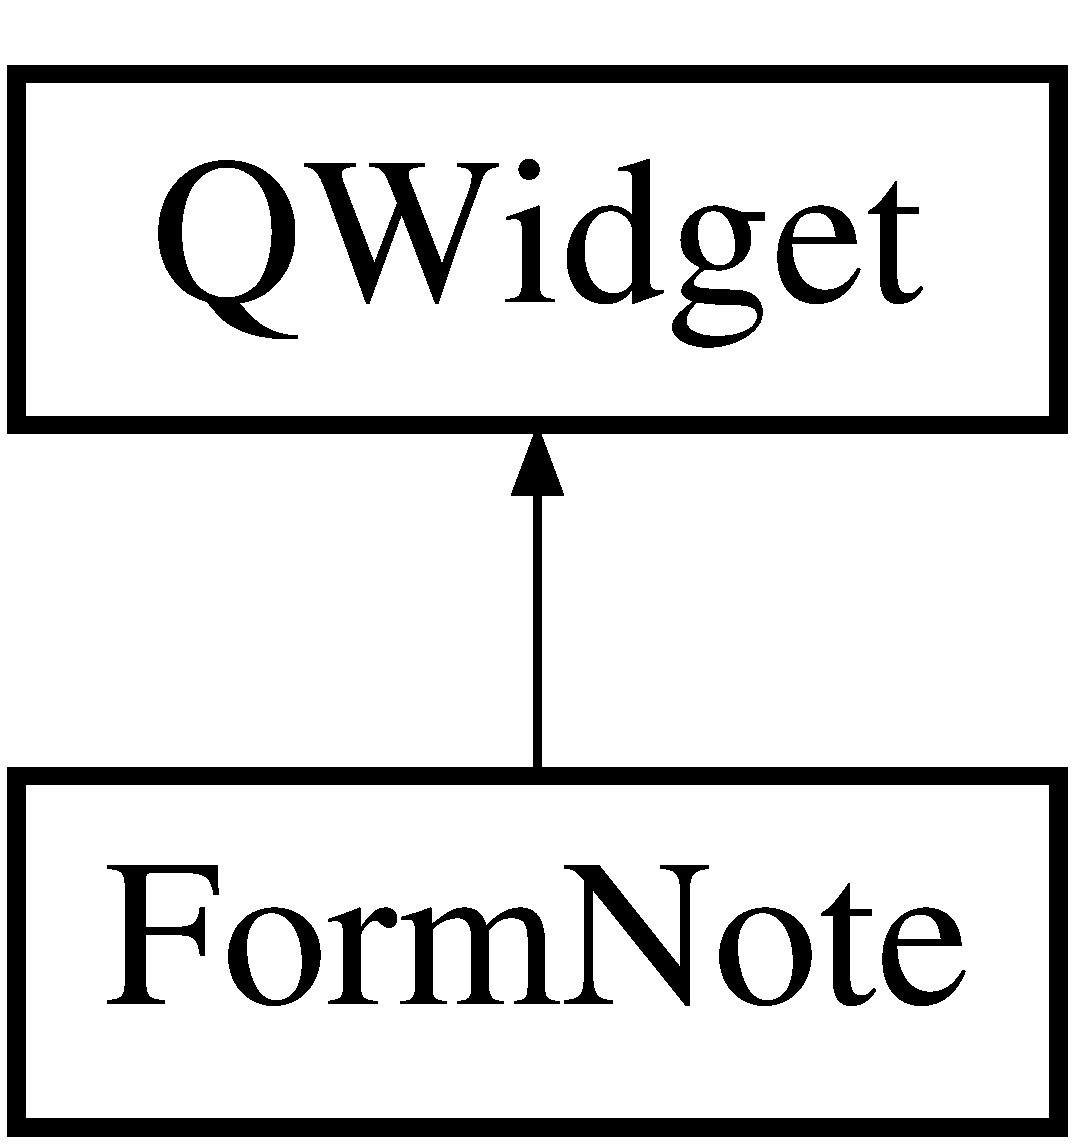
\includegraphics[height=2.000000cm]{class_form_note}
\end{center}
\end{figure}
\subsection*{Public Slots}
\begin{DoxyCompactItemize}
\item 
\mbox{\Hypertarget{class_form_note_a6e4ade87e298737a37407194519f6bdd}\label{class_form_note_a6e4ade87e298737a37407194519f6bdd}} 
void {\bfseries activate\+Buttons} ()
\item 
\mbox{\Hypertarget{class_form_note_a989367d8a01755c740252a5f08610cb6}\label{class_form_note_a989367d8a01755c740252a5f08610cb6}} 
void {\bfseries disable\+Buttons} ()
\item 
\mbox{\Hypertarget{class_form_note_a052d71f4e7c3cae5cb8fa8979a2214c0}\label{class_form_note_a052d71f4e7c3cae5cb8fa8979a2214c0}} 
void {\bfseries save\+Note} ()
\item 
\mbox{\Hypertarget{class_form_note_a1a8becf0976ab645b89546851da17dff}\label{class_form_note_a1a8becf0976ab645b89546851da17dff}} 
void {\bfseries Put\+To\+Trash} ()
\end{DoxyCompactItemize}
\subsection*{Public Member Functions}
\begin{DoxyCompactItemize}
\item 
\mbox{\Hypertarget{class_form_note_aeaa8060643121e5567cb140990e5cbd0}\label{class_form_note_aeaa8060643121e5567cb140990e5cbd0}} 
{\bfseries Form\+Note} (\hyperlink{class_main_window}{Main\+Window} $\ast$mwind, \hyperlink{class_notes_manager}{Notes\+Manager} $\ast$m, unsigned int id, Q\+Widget $\ast$parent=0)
\end{DoxyCompactItemize}


The documentation for this class was generated from the following files\+:\begin{DoxyCompactItemize}
\item 
Documents/\+U\+T\+C/\+G\+I02/\+L\+O21/\+L\+O21/\+Qt\+Version/mainwindow.\+h\item 
Documents/\+U\+T\+C/\+G\+I02/\+L\+O21/\+L\+O21/\+Qt\+Version/mainwindow.\+cpp\end{DoxyCompactItemize}

\hypertarget{class_form_version}{}\section{Form\+Version Class Reference}
\label{class_form_version}\index{Form\+Version@{Form\+Version}}
Inheritance diagram for Form\+Version\+:\begin{figure}[H]
\begin{center}
\leavevmode
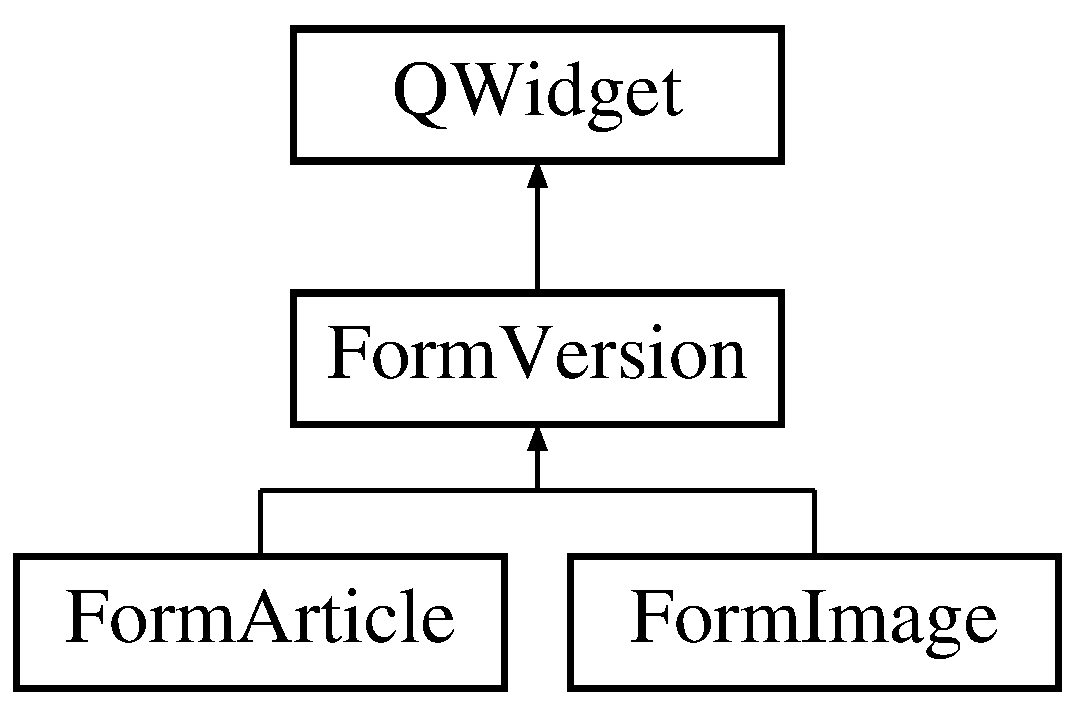
\includegraphics[height=3.000000cm]{class_form_version}
\end{center}
\end{figure}
\subsection*{Public Member Functions}
\begin{DoxyCompactItemize}
\item 
\mbox{\Hypertarget{class_form_version_a8a9de9f27b5558bd1a5b89a076194bea}\label{class_form_version_a8a9de9f27b5558bd1a5b89a076194bea}} 
{\bfseries Form\+Version} (Q\+Widget $\ast$parent=0)
\item 
\mbox{\Hypertarget{class_form_version_a11ab533de81b0930aa8c5e7e53328629}\label{class_form_version_a11ab533de81b0930aa8c5e7e53328629}} 
virtual void {\bfseries save\+Version} (\hyperlink{class_note_version}{Note\+Version} $\ast$)=0
\end{DoxyCompactItemize}


The documentation for this class was generated from the following files\+:\begin{DoxyCompactItemize}
\item 
Documents/\+U\+T\+C/\+G\+I02/\+L\+O21/\+L\+O21/\+Qt\+Version/\hyperlink{noteversion_8h}{noteversion.\+h}\item 
Documents/\+U\+T\+C/\+G\+I02/\+L\+O21/\+L\+O21/\+Qt\+Version/noteversion.\+cpp\end{DoxyCompactItemize}

\hypertarget{class_image}{}\section{Image Class Reference}
\label{class_image}\index{Image@{Image}}
Inheritance diagram for Image\+:\begin{figure}[H]
\begin{center}
\leavevmode
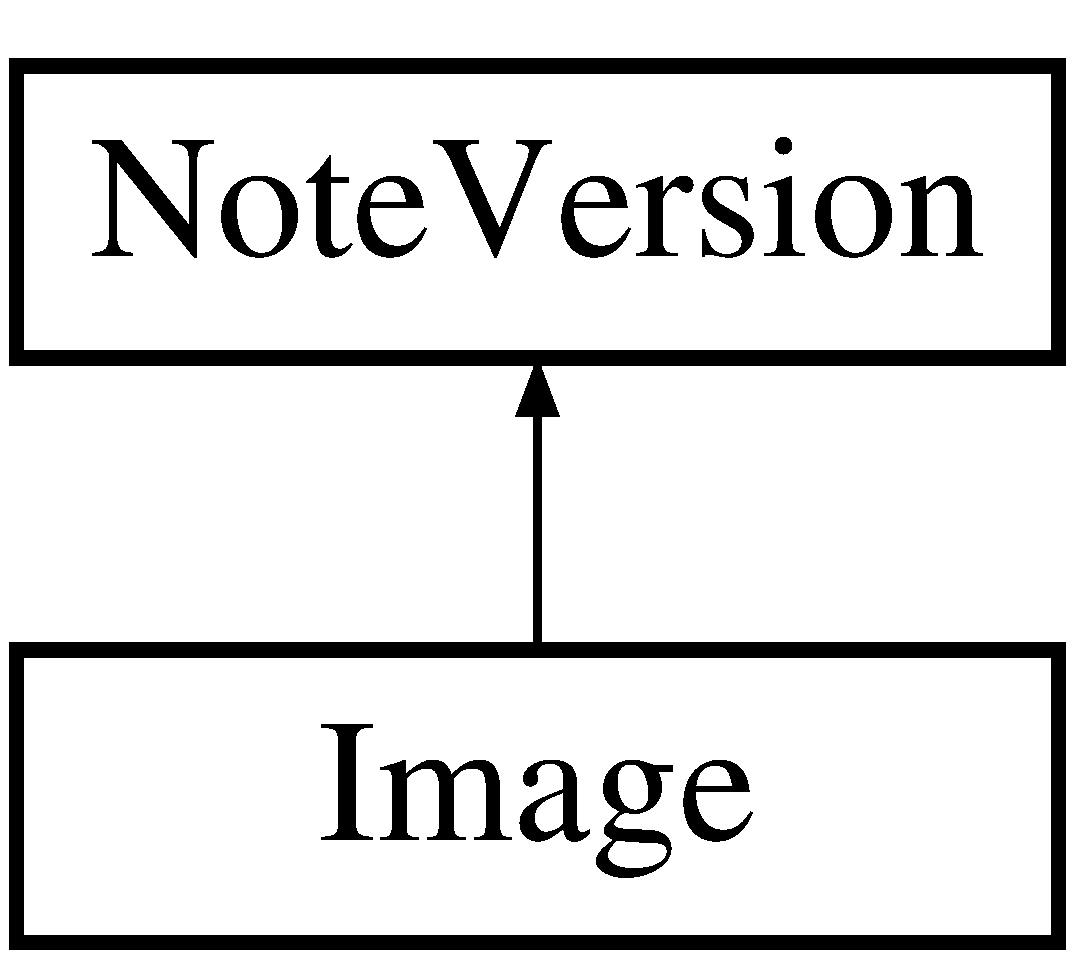
\includegraphics[height=2.000000cm]{class_image}
\end{center}
\end{figure}
\subsection*{Public Member Functions}
\begin{DoxyCompactItemize}
\item 
\hyperlink{class_image_a1072569a682d28333fa03c94efe0c66e}{Image} (const Q\+String \&t=Q\+String(), const Q\+String \&d=Q\+String(), const Q\+String \&f=Q\+String())
\begin{DoxyCompactList}\small\item\em Constructeur de la classe \hyperlink{class_image}{Image}. \end{DoxyCompactList}\item 
\mbox{\Hypertarget{class_image_a570b04dd7ff57e44f508d8a4457e2372}\label{class_image_a570b04dd7ff57e44f508d8a4457e2372}} 
const Q\+String \& \hyperlink{class_image_a570b04dd7ff57e44f508d8a4457e2372}{get\+Description} () const
\begin{DoxyCompactList}\small\item\em accesseur pour obtenir la description d\textquotesingle{}une \hyperlink{class_image}{Image} \end{DoxyCompactList}\item 
\mbox{\Hypertarget{class_image_ac34f9d0352ba64f36e4d2c0a59acf171}\label{class_image_ac34f9d0352ba64f36e4d2c0a59acf171}} 
const Q\+String \& \hyperlink{class_image_ac34f9d0352ba64f36e4d2c0a59acf171}{get\+File} () const
\begin{DoxyCompactList}\small\item\em accesseur pour obtenir le fichier d\textquotesingle{}une \hyperlink{class_image}{Image} \end{DoxyCompactList}\item 
\hyperlink{class_image}{Image} $\ast$ \hyperlink{class_image_a31a754ded7599e3f1a9b83bdcc4437c0}{clone} (unsigned int id) const
\begin{DoxyCompactList}\small\item\em methode clone \end{DoxyCompactList}\item 
\mbox{\Hypertarget{class_image_adee895eaa5e0a96c7d9a63618ac36ef4}\label{class_image_adee895eaa5e0a96c7d9a63618ac36ef4}} 
Q\+String {\bfseries type} () const
\item 
\mbox{\Hypertarget{class_image_a7fadda40fc83245d4e6839c00eac57f2}\label{class_image_a7fadda40fc83245d4e6839c00eac57f2}} 
\hyperlink{class_form_version}{Form\+Version} $\ast$ {\bfseries form\+Version} ()
\end{DoxyCompactItemize}
\subsection*{Friends}
\begin{DoxyCompactItemize}
\item 
\mbox{\Hypertarget{class_image_a93d7e72623acdfa5b079a11fbf2d9f9d}\label{class_image_a93d7e72623acdfa5b079a11fbf2d9f9d}} 
class {\bfseries Note}
\end{DoxyCompactItemize}
\subsection*{Additional Inherited Members}


\subsection{Constructor \& Destructor Documentation}
\mbox{\Hypertarget{class_image_a1072569a682d28333fa03c94efe0c66e}\label{class_image_a1072569a682d28333fa03c94efe0c66e}} 
\index{Image@{Image}!Image@{Image}}
\index{Image@{Image}!Image@{Image}}
\subsubsection{\texorpdfstring{Image()}{Image()}}
{\footnotesize\ttfamily Image\+::\+Image (\begin{DoxyParamCaption}\item[{const Q\+String \&}]{t = {\ttfamily QString()},  }\item[{const Q\+String \&}]{d = {\ttfamily QString()},  }\item[{const Q\+String \&}]{f = {\ttfamily QString()} }\end{DoxyParamCaption})}



Constructeur de la classe \hyperlink{class_image}{Image}. 


\begin{DoxyParams}{Parameters}
{\em t} & titre de l\textquotesingle{}\hyperlink{class_image}{Image} (utilisé par le constructeur de \hyperlink{class_note_version}{Note\+Version}) \\
\hline
{\em d} & description de l\textquotesingle{}\hyperlink{class_image}{Image} \\
\hline
{\em f} & fichier de l\textquotesingle{}\hyperlink{class_image}{Image} \\
\hline
\end{DoxyParams}


\subsection{Member Function Documentation}
\mbox{\Hypertarget{class_image_a31a754ded7599e3f1a9b83bdcc4437c0}\label{class_image_a31a754ded7599e3f1a9b83bdcc4437c0}} 
\index{Image@{Image}!clone@{clone}}
\index{clone@{clone}!Image@{Image}}
\subsubsection{\texorpdfstring{clone()}{clone()}}
{\footnotesize\ttfamily \hyperlink{class_image}{Image} $\ast$ Image\+::clone (\begin{DoxyParamCaption}\item[{unsigned int}]{id }\end{DoxyParamCaption}) const\hspace{0.3cm}{\ttfamily [virtual]}}



methode clone 

\begin{DoxyReturn}{Returns}
un pointeur de \hyperlink{class_image}{Image} sur le clone de l\textquotesingle{}image grâce à l\textquotesingle{}id 
\end{DoxyReturn}

\begin{DoxyParams}{Parameters}
{\em id} & L\textquotesingle{}id de l\textquotesingle{}image que l\textquotesingle{}on souhaite cloner \\
\hline
\end{DoxyParams}


Implements \hyperlink{class_note_version_a7eb23a52291ec623b9bc1b6fe3e86c5a}{Note\+Version}.



The documentation for this class was generated from the following files\+:\begin{DoxyCompactItemize}
\item 
Documents/\+U\+T\+C/\+G\+I02/\+L\+O21/\+L\+O21/\+Qt\+Version/\hyperlink{noteversion_8h}{noteversion.\+h}\item 
Documents/\+U\+T\+C/\+G\+I02/\+L\+O21/\+L\+O21/\+Qt\+Version/noteversion.\+cpp\end{DoxyCompactItemize}

\hypertarget{class_main_window}{}\section{Main\+Window Class Reference}
\label{class_main_window}\index{Main\+Window@{Main\+Window}}
Inheritance diagram for Main\+Window\+:\begin{figure}[H]
\begin{center}
\leavevmode
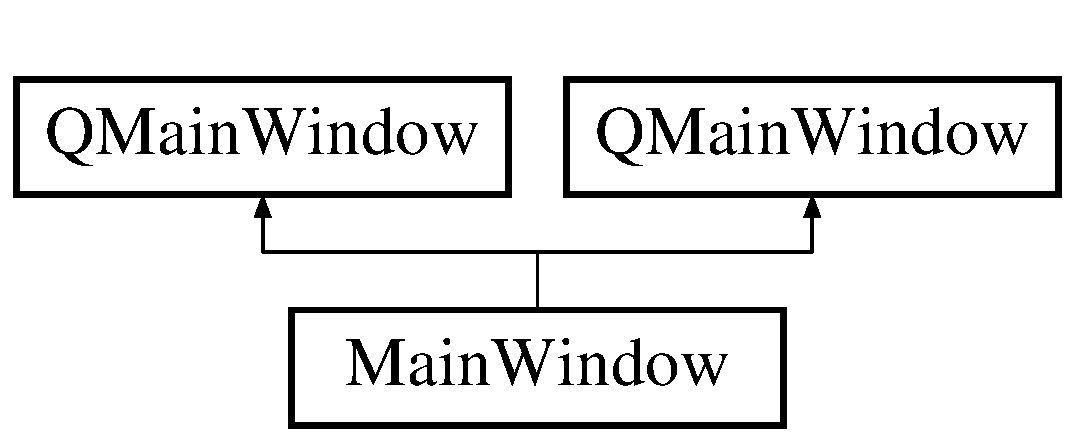
\includegraphics[height=2.000000cm]{class_main_window}
\end{center}
\end{figure}
\subsection*{Public Member Functions}
\begin{DoxyCompactItemize}
\item 
\mbox{\Hypertarget{class_main_window_a8b244be8b7b7db1b08de2a2acb9409db}\label{class_main_window_a8b244be8b7b7db1b08de2a2acb9409db}} 
{\bfseries Main\+Window} (Q\+Widget $\ast$parent=0)
\item 
\mbox{\Hypertarget{class_main_window_a15dd15d76c5b7e9ef6078dca836da2e9}\label{class_main_window_a15dd15d76c5b7e9ef6078dca836da2e9}} 
{\bfseries Main\+Window} (\hyperlink{class_notes_manager}{Notes\+Manager} $\ast$m, \hyperlink{class_trash}{Trash} $\ast$t, Q\+Widget $\ast$parent=0)
\item 
\mbox{\Hypertarget{class_main_window_a5fe2f79d1669b8404a059542ecaf011b}\label{class_main_window_a5fe2f79d1669b8404a059542ecaf011b}} 
void {\bfseries load\+Active\+Notes} ()
\item 
\mbox{\Hypertarget{class_main_window_aebff467c9b6fc051e2f77546a100f3e5}\label{class_main_window_aebff467c9b6fc051e2f77546a100f3e5}} 
void {\bfseries unload\+Active\+Notes} ()
\item 
\mbox{\Hypertarget{class_main_window_ab27297114529e4c16d6d8d7a54927a0e}\label{class_main_window_ab27297114529e4c16d6d8d7a54927a0e}} 
void {\bfseries refresh} ()
\item 
\mbox{\Hypertarget{class_main_window_aca9c0a991a4a3591d9e705442fb06adc}\label{class_main_window_aca9c0a991a4a3591d9e705442fb06adc}} 
void {\bfseries unload\+Trashed\+Notes} ()
\item 
\mbox{\Hypertarget{class_main_window_aef33129c84ee03ef6e7070712e6de651}\label{class_main_window_aef33129c84ee03ef6e7070712e6de651}} 
void {\bfseries load\+Trashed\+Notes} ()
\item 
\mbox{\Hypertarget{class_main_window_aecb2d69ac160ebf1db460d6854b14182}\label{class_main_window_aecb2d69ac160ebf1db460d6854b14182}} 
void {\bfseries restore\+Note} ()
\item 
\mbox{\Hypertarget{class_main_window_a3a169e9346099a7a81aa2d3bee01525d}\label{class_main_window_a3a169e9346099a7a81aa2d3bee01525d}} 
void {\bfseries delete\+Note} ()
\end{DoxyCompactItemize}


The documentation for this class was generated from the following files\+:\begin{DoxyCompactItemize}
\item 
Documents/\+G\+I02/\+L\+O21/\+Projet/\+L\+O21/\+Qt\+Version/Interface\+J.\+h\item 
Documents/\+G\+I02/\+L\+O21/\+Projet/\+L\+O21/\+Qt\+Version/mainwindow.\+h\item 
Documents/\+G\+I02/\+L\+O21/\+Projet/\+L\+O21/\+Qt\+Version/interface\+J.\+cpp\item 
Documents/\+G\+I02/\+L\+O21/\+Projet/\+L\+O21/\+Qt\+Version/mainwindow.\+cpp\end{DoxyCompactItemize}

\hypertarget{class_note}{}\section{Note Class Reference}
\label{class_note}\index{Note@{Note}}


{\ttfamily \#include $<$note.\+h$>$}

\subsection*{Public Member Functions}
\begin{DoxyCompactItemize}
\item 
\mbox{\Hypertarget{class_note_a40ceb432567359e26bf865c890323f30}\label{class_note_a40ceb432567359e26bf865c890323f30}} 
unsigned int \hyperlink{class_note_a40ceb432567359e26bf865c890323f30}{get\+Id\+Note} () const
\begin{DoxyCompactList}\small\item\em accesseur pour obtenir l\textquotesingle{}id d\textquotesingle{}une note \end{DoxyCompactList}\item 
\mbox{\Hypertarget{class_note_a598ee9613bcc6a062c79792cb7025ee9}\label{class_note_a598ee9613bcc6a062c79792cb7025ee9}} 
const \hyperlink{class_date}{Date} \& \hyperlink{class_note_a598ee9613bcc6a062c79792cb7025ee9}{get\+Date\+Crea} () const
\begin{DoxyCompactList}\small\item\em accesseur pour obtenir la date d\textquotesingle{}une note \end{DoxyCompactList}\item 
\mbox{\Hypertarget{class_note_a58bc3eb637d334bde81b9f35ad4c7ccc}\label{class_note_a58bc3eb637d334bde81b9f35ad4c7ccc}} 
\hyperlink{note_8h_adc6e5733fc3c22f0a7b2914188c49c90}{state} \hyperlink{class_note_a58bc3eb637d334bde81b9f35ad4c7ccc}{get\+Note\+State} ()
\begin{DoxyCompactList}\small\item\em accesseur pour obtenir l\textquotesingle{}état d\textquotesingle{}une note \end{DoxyCompactList}\item 
int \hyperlink{class_note_a47714d07648fd428150405085ac612b1}{add\+Note\+Version} (const \hyperlink{class_note_version}{Note\+Version} \&n)
\begin{DoxyCompactList}\small\item\em Méthode pour ajouter une version à une note. \end{DoxyCompactList}\item 
\mbox{\Hypertarget{class_note_a725bfabf6f31b9572c80c94435e2ab41}\label{class_note_a725bfabf6f31b9572c80c94435e2ab41}} 
int \hyperlink{class_note_a725bfabf6f31b9572c80c94435e2ab41}{copy\+Latest\+Version} ()
\begin{DoxyCompactList}\small\item\em Méthode pour avoir l\textquotesingle{}id de la dernière version d\textquotesingle{}une note. \end{DoxyCompactList}\item 
\hyperlink{class_note_version}{Note\+Version} \& \hyperlink{class_note_ae60bb551ea83c20362c3d3ef1f28118c}{get\+Note\+Version} (unsigned int id) const
\begin{DoxyCompactList}\small\item\em Méthode pour avoir la version d\textquotesingle{}une note à partir de son id. \end{DoxyCompactList}\item 
\mbox{\Hypertarget{class_note_a3331744580a5de2d4c04ade505d675b8}\label{class_note_a3331744580a5de2d4c04ade505d675b8}} 
\hyperlink{class_note_version}{Note\+Version} \& \hyperlink{class_note_a3331744580a5de2d4c04ade505d675b8}{get\+Latest\+Note\+Version} ()
\begin{DoxyCompactList}\small\item\em Méthode pour avoir la version actuelle d\textquotesingle{}une note. \end{DoxyCompactList}\end{DoxyCompactItemize}
\subsection*{Friends}
\begin{DoxyCompactItemize}
\item 
\mbox{\Hypertarget{class_note_a017a5144e8cfa6087305055ab968ef41}\label{class_note_a017a5144e8cfa6087305055ab968ef41}} 
class {\bfseries Notes\+Manager}
\item 
\mbox{\Hypertarget{class_note_aa5b165af6155aa1d6b8c634a27eae73f}\label{class_note_aa5b165af6155aa1d6b8c634a27eae73f}} 
class {\bfseries Trash}
\end{DoxyCompactItemize}


\subsection{Detailed Description}
La classe \hyperlink{class_notes_manager}{Notes\+Manager} est un singleton car il ne peut exister qu\textquotesingle{}une seule instance. 

\subsection{Member Function Documentation}
\mbox{\Hypertarget{class_note_a47714d07648fd428150405085ac612b1}\label{class_note_a47714d07648fd428150405085ac612b1}} 
\index{Note@{Note}!add\+Note\+Version@{add\+Note\+Version}}
\index{add\+Note\+Version@{add\+Note\+Version}!Note@{Note}}
\subsubsection{\texorpdfstring{add\+Note\+Version()}{addNoteVersion()}}
{\footnotesize\ttfamily int Note\+::add\+Note\+Version (\begin{DoxyParamCaption}\item[{const \hyperlink{class_note_version}{Note\+Version} \&}]{n }\end{DoxyParamCaption})}



Méthode pour ajouter une version à une note. 


\begin{DoxyParams}{Parameters}
{\em n} & Reference sur une version d\textquotesingle{}une note \\
\hline
\end{DoxyParams}
\mbox{\Hypertarget{class_note_ae60bb551ea83c20362c3d3ef1f28118c}\label{class_note_ae60bb551ea83c20362c3d3ef1f28118c}} 
\index{Note@{Note}!get\+Note\+Version@{get\+Note\+Version}}
\index{get\+Note\+Version@{get\+Note\+Version}!Note@{Note}}
\subsubsection{\texorpdfstring{get\+Note\+Version()}{getNoteVersion()}}
{\footnotesize\ttfamily \hyperlink{class_note_version}{Note\+Version} \& Note\+::get\+Note\+Version (\begin{DoxyParamCaption}\item[{unsigned int}]{id }\end{DoxyParamCaption}) const}



Méthode pour avoir la version d\textquotesingle{}une note à partir de son id. 


\begin{DoxyParams}{Parameters}
{\em id} & id de la version de la note \\
\hline
\end{DoxyParams}


The documentation for this class was generated from the following files\+:\begin{DoxyCompactItemize}
\item 
Documents/\+G\+I02/\+L\+O21/\+Projet/\+L\+O21/\+Qt\+Version/\hyperlink{note_8h}{note.\+h}\item 
Documents/\+G\+I02/\+L\+O21/\+Projet/\+L\+O21/\+Qt\+Version/note.\+cpp\end{DoxyCompactItemize}

\hypertarget{class_notes_editor}{}\section{Notes\+Editor Class Reference}
\label{class_notes_editor}\index{Notes\+Editor@{Notes\+Editor}}


The documentation for this class was generated from the following file\+:\begin{DoxyCompactItemize}
\item 
Documents/\+G\+I02/\+L\+O21/\+Projet/\+L\+O21/\+Qt\+Version/noteseditor.\+h\end{DoxyCompactItemize}

\hypertarget{class_notes_manager}{}\section{Notes\+Manager Class Reference}
\label{class_notes_manager}\index{Notes\+Manager@{Notes\+Manager}}
\subsection*{Public Member Functions}
\begin{DoxyCompactItemize}
\item 
void \hyperlink{class_notes_manager_aaa57ac37417937f81173c0ad93298a2a}{set\+Filename} (const Q\+String \&str)
\begin{DoxyCompactList}\small\item\em Défini le nom de l\textquotesingle{}instance \hyperlink{class_notes_manager}{Notes\+Manager}. \end{DoxyCompactList}\item 
int \hyperlink{class_notes_manager_ac94f24bd2797edf14146d9caa1a50f36}{add\+Note} ()
\begin{DoxyCompactList}\small\item\em Ajoute une \hyperlink{class_note}{Note}. \end{DoxyCompactList}\item 
void \hyperlink{class_notes_manager_a2155d076ae6e1044e621f90ebc669466}{add\+Existing\+Note} (\hyperlink{class_note}{Note} $\ast$n)
\begin{DoxyCompactList}\small\item\em Ajoute une note déjà existante. \end{DoxyCompactList}\item 
\hyperlink{class_note}{Note} \& \hyperlink{class_notes_manager_a559c0b690aa23fb568b4a8e53a6f51cc}{get\+Note} (unsigned int id)
\begin{DoxyCompactList}\small\item\em Obtenir une note à partir de son id. \end{DoxyCompactList}\item 
const std\+::vector$<$ \hyperlink{class_note}{Note} $\ast$ $>$ \& \hyperlink{class_notes_manager_a423e040490fa4a8244acd90c754fe7b5}{get\+List\+Notes} () const
\begin{DoxyCompactList}\small\item\em Obtenir la list de toutes les notes. \end{DoxyCompactList}\item 
void \hyperlink{class_notes_manager_a69ef4ff2eb05ec962c7f8cb80d0d15d3}{put\+To\+Trash} (unsigned int id)
\begin{DoxyCompactList}\small\item\em Mettre une note à la corbeille. \end{DoxyCompactList}\item 
void \hyperlink{class_notes_manager_ad271bd7f8079b01b04a32b886b498bac}{save} () const
\begin{DoxyCompactList}\small\item\em Sauvegarder la liste de Notes. \end{DoxyCompactList}\item 
void \hyperlink{class_notes_manager_ad4fb2de50633dd25b71024343341cd64}{load} ()
\begin{DoxyCompactList}\small\item\em Charger la liste de Notes. \end{DoxyCompactList}\end{DoxyCompactItemize}
\subsection*{Static Public Member Functions}
\begin{DoxyCompactItemize}
\item 
static \hyperlink{class_notes_manager}{Notes\+Manager} \& \hyperlink{class_notes_manager_a62868e66f00cf991822c7ffd5e751b31}{get\+Instance} ()
\begin{DoxyCompactList}\small\item\em Constructeur de l\textquotesingle{}unique instance du singleton. \end{DoxyCompactList}\end{DoxyCompactItemize}


\subsection{Member Function Documentation}
\mbox{\Hypertarget{class_notes_manager_a2155d076ae6e1044e621f90ebc669466}\label{class_notes_manager_a2155d076ae6e1044e621f90ebc669466}} 
\index{Notes\+Manager@{Notes\+Manager}!add\+Existing\+Note@{add\+Existing\+Note}}
\index{add\+Existing\+Note@{add\+Existing\+Note}!Notes\+Manager@{Notes\+Manager}}
\subsubsection{\texorpdfstring{add\+Existing\+Note()}{addExistingNote()}}
{\footnotesize\ttfamily void Notes\+Manager\+::add\+Existing\+Note (\begin{DoxyParamCaption}\item[{\hyperlink{class_note}{Note} $\ast$}]{n }\end{DoxyParamCaption})}



Ajoute une note déjà existante. 


\begin{DoxyParams}{Parameters}
{\em n} & Pointeur sur la note à ajouter \\
\hline
\end{DoxyParams}
\mbox{\Hypertarget{class_notes_manager_ac94f24bd2797edf14146d9caa1a50f36}\label{class_notes_manager_ac94f24bd2797edf14146d9caa1a50f36}} 
\index{Notes\+Manager@{Notes\+Manager}!add\+Note@{add\+Note}}
\index{add\+Note@{add\+Note}!Notes\+Manager@{Notes\+Manager}}
\subsubsection{\texorpdfstring{add\+Note()}{addNote()}}
{\footnotesize\ttfamily int Notes\+Manager\+::add\+Note (\begin{DoxyParamCaption}{ }\end{DoxyParamCaption})}



Ajoute une \hyperlink{class_note}{Note}. 

La nouvelle note possède un nouvel identifiant qui est celui de la dernière note + 1. La nouvelle note est vide à sa création \mbox{\Hypertarget{class_notes_manager_a62868e66f00cf991822c7ffd5e751b31}\label{class_notes_manager_a62868e66f00cf991822c7ffd5e751b31}} 
\index{Notes\+Manager@{Notes\+Manager}!get\+Instance@{get\+Instance}}
\index{get\+Instance@{get\+Instance}!Notes\+Manager@{Notes\+Manager}}
\subsubsection{\texorpdfstring{get\+Instance()}{getInstance()}}
{\footnotesize\ttfamily static \hyperlink{class_notes_manager}{Notes\+Manager}\& Notes\+Manager\+::get\+Instance (\begin{DoxyParamCaption}{ }\end{DoxyParamCaption})\hspace{0.3cm}{\ttfamily [inline]}, {\ttfamily [static]}}



Constructeur de l\textquotesingle{}unique instance du singleton. 

c\textquotesingle{}est une méthode statique \mbox{\Hypertarget{class_notes_manager_a423e040490fa4a8244acd90c754fe7b5}\label{class_notes_manager_a423e040490fa4a8244acd90c754fe7b5}} 
\index{Notes\+Manager@{Notes\+Manager}!get\+List\+Notes@{get\+List\+Notes}}
\index{get\+List\+Notes@{get\+List\+Notes}!Notes\+Manager@{Notes\+Manager}}
\subsubsection{\texorpdfstring{get\+List\+Notes()}{getListNotes()}}
{\footnotesize\ttfamily const std\+::vector$<$\hyperlink{class_note}{Note}$\ast$$>$\& Notes\+Manager\+::get\+List\+Notes (\begin{DoxyParamCaption}{ }\end{DoxyParamCaption}) const\hspace{0.3cm}{\ttfamily [inline]}}



Obtenir la list de toutes les notes. 

Cette méthode retourne la liste de toutes les notes stockées dans le vecteur \mbox{\Hypertarget{class_notes_manager_a559c0b690aa23fb568b4a8e53a6f51cc}\label{class_notes_manager_a559c0b690aa23fb568b4a8e53a6f51cc}} 
\index{Notes\+Manager@{Notes\+Manager}!get\+Note@{get\+Note}}
\index{get\+Note@{get\+Note}!Notes\+Manager@{Notes\+Manager}}
\subsubsection{\texorpdfstring{get\+Note()}{getNote()}}
{\footnotesize\ttfamily \hyperlink{class_note}{Note} \& Notes\+Manager\+::get\+Note (\begin{DoxyParamCaption}\item[{unsigned int}]{id }\end{DoxyParamCaption})}



Obtenir une note à partir de son id. 


\begin{DoxyParams}{Parameters}
{\em id} & Id de la note que l\textquotesingle{}on souhaite obtenir \\
\hline
\end{DoxyParams}
\mbox{\Hypertarget{class_notes_manager_ad4fb2de50633dd25b71024343341cd64}\label{class_notes_manager_ad4fb2de50633dd25b71024343341cd64}} 
\index{Notes\+Manager@{Notes\+Manager}!load@{load}}
\index{load@{load}!Notes\+Manager@{Notes\+Manager}}
\subsubsection{\texorpdfstring{load()}{load()}}
{\footnotesize\ttfamily void Notes\+Manager\+::load (\begin{DoxyParamCaption}{ }\end{DoxyParamCaption})}



Charger la liste de Notes. 

Cette méthode charge le vecteur de notes à partir d\textquotesingle{}un fichier xml à l\textquotesingle{}ouverture de l\textquotesingle{}application \mbox{\Hypertarget{class_notes_manager_a69ef4ff2eb05ec962c7f8cb80d0d15d3}\label{class_notes_manager_a69ef4ff2eb05ec962c7f8cb80d0d15d3}} 
\index{Notes\+Manager@{Notes\+Manager}!put\+To\+Trash@{put\+To\+Trash}}
\index{put\+To\+Trash@{put\+To\+Trash}!Notes\+Manager@{Notes\+Manager}}
\subsubsection{\texorpdfstring{put\+To\+Trash()}{putToTrash()}}
{\footnotesize\ttfamily void Notes\+Manager\+::put\+To\+Trash (\begin{DoxyParamCaption}\item[{unsigned int}]{id }\end{DoxyParamCaption})}



Mettre une note à la corbeille. 

Cette méthode permet de mettre une note qui est supprimée à la corbeille. Si nous avons le temps cette méthode verifiera que la note en question n\textquotesingle{}est pas dans un couple de la relation référence. Le cas échéant elle serait alors archivée et non mise à la corbeille tant qu\textquotesingle{}elle est dans ce couple. Si la deuxième note qui forme le couple avec la première venait elle aussi à être supprimée elle serait alors toutes les deux mises à la corbeille. 
\begin{DoxyParams}{Parameters}
{\em id} & Id de la note que l\textquotesingle{}on souhaite mettre à la corbeille \\
\hline
\end{DoxyParams}
\mbox{\Hypertarget{class_notes_manager_ad271bd7f8079b01b04a32b886b498bac}\label{class_notes_manager_ad271bd7f8079b01b04a32b886b498bac}} 
\index{Notes\+Manager@{Notes\+Manager}!save@{save}}
\index{save@{save}!Notes\+Manager@{Notes\+Manager}}
\subsubsection{\texorpdfstring{save()}{save()}}
{\footnotesize\ttfamily void Notes\+Manager\+::save (\begin{DoxyParamCaption}{ }\end{DoxyParamCaption}) const}



Sauvegarder la liste de Notes. 

Cette méthode sauvegarde le vecteur de notes dans un fichier xml à la fermeture de l\textquotesingle{}application \mbox{\Hypertarget{class_notes_manager_aaa57ac37417937f81173c0ad93298a2a}\label{class_notes_manager_aaa57ac37417937f81173c0ad93298a2a}} 
\index{Notes\+Manager@{Notes\+Manager}!set\+Filename@{set\+Filename}}
\index{set\+Filename@{set\+Filename}!Notes\+Manager@{Notes\+Manager}}
\subsubsection{\texorpdfstring{set\+Filename()}{setFilename()}}
{\footnotesize\ttfamily void Notes\+Manager\+::set\+Filename (\begin{DoxyParamCaption}\item[{const Q\+String \&}]{str }\end{DoxyParamCaption})\hspace{0.3cm}{\ttfamily [inline]}}



Défini le nom de l\textquotesingle{}instance \hyperlink{class_notes_manager}{Notes\+Manager}. 


\begin{DoxyParams}{Parameters}
{\em std} & Nom de l\textquotesingle{}instance \\
\hline
\end{DoxyParams}


The documentation for this class was generated from the following files\+:\begin{DoxyCompactItemize}
\item 
Documents/\+U\+T\+C/\+G\+I02/\+L\+O21/\+L\+O21/\+Qt\+Version/\hyperlink{notesmanager_8h}{notesmanager.\+h}\item 
Documents/\+U\+T\+C/\+G\+I02/\+L\+O21/\+L\+O21/\+Qt\+Version/notesmanager.\+cpp\end{DoxyCompactItemize}

\hypertarget{class_note_version}{}\section{Note\+Version Class Reference}
\label{class_note_version}\index{Note\+Version@{Note\+Version}}


{\ttfamily \#include $<$noteversion.\+h$>$}

Inheritance diagram for Note\+Version\+:\begin{figure}[H]
\begin{center}
\leavevmode
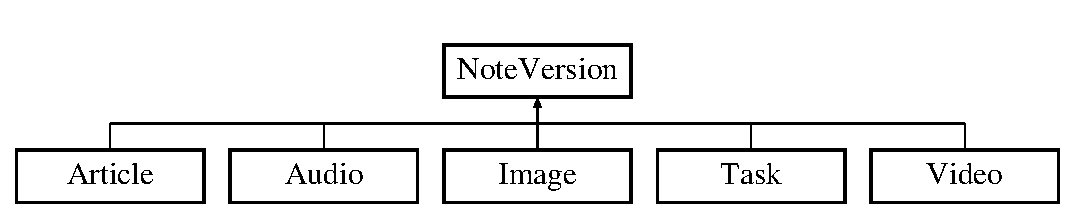
\includegraphics[height=2.000000cm]{class_note_version}
\end{center}
\end{figure}
\subsection*{Public Member Functions}
\begin{DoxyCompactItemize}
\item 
\hyperlink{class_note_version_ad4404543d7a26d44a5a40690d262de5f}{Note\+Version} (unsigned int v, const Q\+String \&t)
\begin{DoxyCompactList}\small\item\em Constructeur de la classe \hyperlink{class_note_version}{Note\+Version}. \end{DoxyCompactList}\item 
\mbox{\Hypertarget{class_note_version_a8277b7b1b364d999accd276ef8107e4c}\label{class_note_version_a8277b7b1b364d999accd276ef8107e4c}} 
const Q\+String \& \hyperlink{class_note_version_a8277b7b1b364d999accd276ef8107e4c}{get\+Title} () const
\begin{DoxyCompactList}\small\item\em accesseur pour obtenir le titre d\textquotesingle{}une version d\textquotesingle{}une note \end{DoxyCompactList}\item 
void \hyperlink{class_note_version_a1b9f3da6615a30ce9cda5c884559f37a}{set\+Title} (const Q\+String \&str)
\begin{DoxyCompactList}\small\item\em méthode pour appliquer un titre à une version d\textquotesingle{}une note \end{DoxyCompactList}\item 
\mbox{\Hypertarget{class_note_version_aee1009d4e2ff0d26cc24350846685c25}\label{class_note_version_aee1009d4e2ff0d26cc24350846685c25}} 
const \hyperlink{class_date}{Date} \& \hyperlink{class_note_version_aee1009d4e2ff0d26cc24350846685c25}{get\+Date\+Edit} () const
\begin{DoxyCompactList}\small\item\em accesseur pour obtenir la date d\textquotesingle{}édition d\textquotesingle{}une version d\textquotesingle{}une note \end{DoxyCompactList}\item 
void \hyperlink{class_note_version_ae8b130460a53c39631ffa283387067f5}{set\+Date\+Edit} (const \hyperlink{class_date}{Date} \&d)
\begin{DoxyCompactList}\small\item\em méthode pour appliquer une date d\textquotesingle{}édition à une version d\textquotesingle{}une note \end{DoxyCompactList}\item 
\mbox{\Hypertarget{class_note_version_a45dcb249d3bc6ce68f8c9dcabf153187}\label{class_note_version_a45dcb249d3bc6ce68f8c9dcabf153187}} 
unsigned int \hyperlink{class_note_version_a45dcb249d3bc6ce68f8c9dcabf153187}{get\+Id\+Version} () const
\begin{DoxyCompactList}\small\item\em accesseur pour obtenir l\textquotesingle{}id d\textquotesingle{}une version d\textquotesingle{}une note \end{DoxyCompactList}\item 
virtual \hyperlink{class_note_version_a84b32b9c97fa1de8b37b1170b9453f00}{$\sim$\+Note\+Version} ()
\begin{DoxyCompactList}\small\item\em destructeur d\textquotesingle{}une version d\textquotesingle{}une note \end{DoxyCompactList}\item 
virtual \hyperlink{class_note_version}{Note\+Version} $\ast$ \hyperlink{class_note_version_a7eb23a52291ec623b9bc1b6fe3e86c5a}{clone} (unsigned int id) const =0
\begin{DoxyCompactList}\small\item\em methode clone \end{DoxyCompactList}\item 
\mbox{\Hypertarget{class_note_version_a950a828eafaae43fff4c37d990d3a4cc}\label{class_note_version_a950a828eafaae43fff4c37d990d3a4cc}} 
virtual Q\+String {\bfseries type} () const =0
\item 
\mbox{\Hypertarget{class_note_version_a18ab9b2f07fb4a832218ca30db27e9bd}\label{class_note_version_a18ab9b2f07fb4a832218ca30db27e9bd}} 
virtual \hyperlink{class_form_version}{Form\+Version} $\ast$ {\bfseries form\+Version} ()=0
\end{DoxyCompactItemize}
\subsection*{Protected Attributes}
\begin{DoxyCompactItemize}
\item 
\mbox{\Hypertarget{class_note_version_a933ace1d0a9c02d3c58dd4a905629adc}\label{class_note_version_a933ace1d0a9c02d3c58dd4a905629adc}} 
unsigned int {\bfseries id\+Version}
\item 
\mbox{\Hypertarget{class_note_version_ac1ccf3cfef8c72bba33ff65d688226fa}\label{class_note_version_ac1ccf3cfef8c72bba33ff65d688226fa}} 
\hyperlink{class_date}{Date} {\bfseries date\+Edit}
\end{DoxyCompactItemize}
\subsection*{Friends}
\begin{DoxyCompactItemize}
\item 
\mbox{\Hypertarget{class_note_version_a93d7e72623acdfa5b079a11fbf2d9f9d}\label{class_note_version_a93d7e72623acdfa5b079a11fbf2d9f9d}} 
class {\bfseries Note}
\end{DoxyCompactItemize}


\subsection{Detailed Description}
Classe amie de \hyperlink{class_note}{Note} 

\subsection{Constructor \& Destructor Documentation}
\mbox{\Hypertarget{class_note_version_ad4404543d7a26d44a5a40690d262de5f}\label{class_note_version_ad4404543d7a26d44a5a40690d262de5f}} 
\index{Note\+Version@{Note\+Version}!Note\+Version@{Note\+Version}}
\index{Note\+Version@{Note\+Version}!Note\+Version@{Note\+Version}}
\subsubsection{\texorpdfstring{Note\+Version()}{NoteVersion()}}
{\footnotesize\ttfamily Note\+Version\+::\+Note\+Version (\begin{DoxyParamCaption}\item[{unsigned int}]{v,  }\item[{const Q\+String \&}]{t }\end{DoxyParamCaption})}



Constructeur de la classe \hyperlink{class_note_version}{Note\+Version}. 


\begin{DoxyParams}{Parameters}
{\em v} & id de la version \\
\hline
{\em t} & titre de la version \\
\hline
\end{DoxyParams}
\mbox{\Hypertarget{class_note_version_a84b32b9c97fa1de8b37b1170b9453f00}\label{class_note_version_a84b32b9c97fa1de8b37b1170b9453f00}} 
\index{Note\+Version@{Note\+Version}!````~Note\+Version@{$\sim$\+Note\+Version}}
\index{````~Note\+Version@{$\sim$\+Note\+Version}!Note\+Version@{Note\+Version}}
\subsubsection{\texorpdfstring{$\sim$\+Note\+Version()}{~NoteVersion()}}
{\footnotesize\ttfamily Note\+Version\+::$\sim$\+Note\+Version (\begin{DoxyParamCaption}{ }\end{DoxyParamCaption})\hspace{0.3cm}{\ttfamily [virtual]}}



destructeur d\textquotesingle{}une version d\textquotesingle{}une note 

il est virtuel 

\subsection{Member Function Documentation}
\mbox{\Hypertarget{class_note_version_a7eb23a52291ec623b9bc1b6fe3e86c5a}\label{class_note_version_a7eb23a52291ec623b9bc1b6fe3e86c5a}} 
\index{Note\+Version@{Note\+Version}!clone@{clone}}
\index{clone@{clone}!Note\+Version@{Note\+Version}}
\subsubsection{\texorpdfstring{clone()}{clone()}}
{\footnotesize\ttfamily virtual \hyperlink{class_note_version}{Note\+Version}$\ast$ Note\+Version\+::clone (\begin{DoxyParamCaption}\item[{unsigned int}]{id }\end{DoxyParamCaption}) const\hspace{0.3cm}{\ttfamily [pure virtual]}}



methode clone 

\begin{DoxyReturn}{Returns}
un pointeur de \hyperlink{class_note_version}{Note\+Version} sur le clone de la version grâce à l\textquotesingle{}id 
\end{DoxyReturn}

\begin{DoxyParams}{Parameters}
{\em id} & L\textquotesingle{}id de la version que l\textquotesingle{}on souhaite cloner \\
\hline
\end{DoxyParams}


Implemented in \hyperlink{class_video_a505ceb0063f73cf8dd06bc6c6ff72c5d}{Video}, \hyperlink{class_audio_ae389c3ddd81187769876a1b1790be587}{Audio}, \hyperlink{class_image_a31a754ded7599e3f1a9b83bdcc4437c0}{Image}, \hyperlink{class_task_a1bbd4cedca0617ce64237e90af5a797a}{Task}, and \hyperlink{class_article_a78188a4d3c5b071caf13db46ecdc32b9}{Article}.

\mbox{\Hypertarget{class_note_version_ae8b130460a53c39631ffa283387067f5}\label{class_note_version_ae8b130460a53c39631ffa283387067f5}} 
\index{Note\+Version@{Note\+Version}!set\+Date\+Edit@{set\+Date\+Edit}}
\index{set\+Date\+Edit@{set\+Date\+Edit}!Note\+Version@{Note\+Version}}
\subsubsection{\texorpdfstring{set\+Date\+Edit()}{setDateEdit()}}
{\footnotesize\ttfamily void Note\+Version\+::set\+Date\+Edit (\begin{DoxyParamCaption}\item[{const \hyperlink{class_date}{Date} \&}]{d }\end{DoxyParamCaption})}



méthode pour appliquer une date d\textquotesingle{}édition à une version d\textquotesingle{}une note 


\begin{DoxyParams}{Parameters}
{\em d} & \hyperlink{class_date}{Date} d\textquotesingle{}édition d\textquotesingle{}une version \\
\hline
\end{DoxyParams}
\mbox{\Hypertarget{class_note_version_a1b9f3da6615a30ce9cda5c884559f37a}\label{class_note_version_a1b9f3da6615a30ce9cda5c884559f37a}} 
\index{Note\+Version@{Note\+Version}!set\+Title@{set\+Title}}
\index{set\+Title@{set\+Title}!Note\+Version@{Note\+Version}}
\subsubsection{\texorpdfstring{set\+Title()}{setTitle()}}
{\footnotesize\ttfamily void Note\+Version\+::set\+Title (\begin{DoxyParamCaption}\item[{const Q\+String \&}]{str }\end{DoxyParamCaption})}



méthode pour appliquer un titre à une version d\textquotesingle{}une note 


\begin{DoxyParams}{Parameters}
{\em str} & Titre d\textquotesingle{}une version \\
\hline
\end{DoxyParams}


The documentation for this class was generated from the following files\+:\begin{DoxyCompactItemize}
\item 
Documents/\+U\+T\+C/\+G\+I02/\+L\+O21/\+L\+O21/\+Qt\+Version/\hyperlink{noteversion_8h}{noteversion.\+h}\item 
Documents/\+U\+T\+C/\+G\+I02/\+L\+O21/\+L\+O21/\+Qt\+Version/noteversion.\+cpp\end{DoxyCompactItemize}

\hypertarget{class_note_version_factory}{}\section{Note\+Version\+Factory Class Reference}
\label{class_note_version_factory}\index{Note\+Version\+Factory@{Note\+Version\+Factory}}
Inheritance diagram for Note\+Version\+Factory\+:\begin{figure}[H]
\begin{center}
\leavevmode
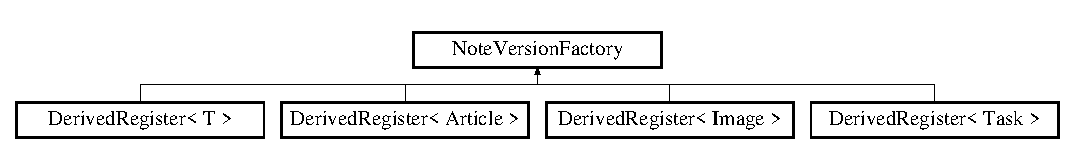
\includegraphics[height=1.627907cm]{class_note_version_factory}
\end{center}
\end{figure}
\subsection*{Public Types}
\begin{DoxyCompactItemize}
\item 
\mbox{\Hypertarget{class_note_version_factory_a5ee840b77e479136a07806129c4c90ef}\label{class_note_version_factory_a5ee840b77e479136a07806129c4c90ef}} 
typedef std\+::map$<$ Q\+String, \hyperlink{class_note_version}{Note\+Version} $\ast$($\ast$)()$>$ {\bfseries map\+\_\+type}
\end{DoxyCompactItemize}
\subsection*{Static Public Member Functions}
\begin{DoxyCompactItemize}
\item 
\mbox{\Hypertarget{class_note_version_factory_a4d4f158a1bf99ff9d88a4008ea7a31db}\label{class_note_version_factory_a4d4f158a1bf99ff9d88a4008ea7a31db}} 
static map\+\_\+type $\ast$ {\bfseries get\+Map} ()
\item 
\mbox{\Hypertarget{class_note_version_factory_a332c745461441d4174608430789b5838}\label{class_note_version_factory_a332c745461441d4174608430789b5838}} 
static \hyperlink{class_note_version}{Note\+Version} $\ast$ {\bfseries create\+Instance} (const Q\+String \&s)
\end{DoxyCompactItemize}


The documentation for this class was generated from the following files\+:\begin{DoxyCompactItemize}
\item 
Documents/\+G\+I02/\+L\+O21/\+Projet/\+L\+O21/\+Qt\+Version/\hyperlink{noteversion_8h}{noteversion.\+h}\item 
Documents/\+G\+I02/\+L\+O21/\+Projet/\+L\+O21/\+Qt\+Version/noteversion.\+cpp\end{DoxyCompactItemize}

\hypertarget{class_relation}{}\section{Relation Class Reference}
\label{class_relation}\index{Relation@{Relation}}
\subsection*{Public Member Functions}
\begin{DoxyCompactItemize}
\item 
\mbox{\Hypertarget{class_relation_ac80a2dddfc48008d40d5c0f5912c91fb}\label{class_relation_ac80a2dddfc48008d40d5c0f5912c91fb}} 
{\bfseries Relation} (const Q\+String \&t, const Q\+String \&d, bool o=true)
\item 
\mbox{\Hypertarget{class_relation_a8f8e09eebfd18260cf861666bbc158d5}\label{class_relation_a8f8e09eebfd18260cf861666bbc158d5}} 
const Q\+String \& {\bfseries get\+Title} ()
\item 
\mbox{\Hypertarget{class_relation_ab7e57505e988b1edfde861f1b5d932b2}\label{class_relation_ab7e57505e988b1edfde861f1b5d932b2}} 
const Q\+String \& {\bfseries get\+Description} ()
\item 
\mbox{\Hypertarget{class_relation_a6dc8d1bb7a79f02b37e338146bc4048f}\label{class_relation_a6dc8d1bb7a79f02b37e338146bc4048f}} 
bool {\bfseries get\+Orientation} ()
\item 
\mbox{\Hypertarget{class_relation_a6a42a4c0195c6dd8b3c9091a968b2396}\label{class_relation_a6a42a4c0195c6dd8b3c9091a968b2396}} 
void {\bfseries add\+Couple} (\hyperlink{class_couple}{Couple} \&c)
\end{DoxyCompactItemize}


The documentation for this class was generated from the following files\+:\begin{DoxyCompactItemize}
\item 
Documents/\+U\+T\+C/\+G\+I02/\+L\+O21/\+L\+O21/\+Qt\+Version/\hyperlink{relation_8h}{relation.\+h}\item 
Documents/\+U\+T\+C/\+G\+I02/\+L\+O21/\+L\+O21/\+Qt\+Version/relation.\+cpp\end{DoxyCompactItemize}

\hypertarget{class_relations_manager}{}\section{Relations\+Manager Class Reference}
\label{class_relations_manager}\index{Relations\+Manager@{Relations\+Manager}}
\subsection*{Public Member Functions}
\begin{DoxyCompactItemize}
\item 
\mbox{\Hypertarget{class_relations_manager_a8fd9802237ce57d8c0b295291bbcc134}\label{class_relations_manager_a8fd9802237ce57d8c0b295291bbcc134}} 
void {\bfseries add\+Relation} (const Q\+String \&t, const Q\+String \&d, bool o)
\item 
\mbox{\Hypertarget{class_relations_manager_afa0aefdcdf5eb54e667b5fbe84c2cd47}\label{class_relations_manager_afa0aefdcdf5eb54e667b5fbe84c2cd47}} 
const \hyperlink{class_relation}{Relation} $\ast$ {\bfseries get\+Relation} (const Q\+String \&t) const
\item 
\mbox{\Hypertarget{class_relations_manager_aff0b03fb4d5885befbe4a6bbab7cbcac}\label{class_relations_manager_aff0b03fb4d5885befbe4a6bbab7cbcac}} 
void {\bfseries delete\+Relation} (const Q\+String \&t)
\item 
\mbox{\Hypertarget{class_relations_manager_a644ef25d2a85209b8a402e416da21311}\label{class_relations_manager_a644ef25d2a85209b8a402e416da21311}} 
void {\bfseries display\+Relation\+Couples} (const Q\+String \&t, std\+::ostream \&f)
\end{DoxyCompactItemize}
\subsection*{Static Public Member Functions}
\begin{DoxyCompactItemize}
\item 
\mbox{\Hypertarget{class_relations_manager_a21bcc3976b29e50f8689d3c6658d9ce4}\label{class_relations_manager_a21bcc3976b29e50f8689d3c6658d9ce4}} 
static \hyperlink{class_relations_manager}{Relations\+Manager} \& {\bfseries get\+Instance} ()
\end{DoxyCompactItemize}


The documentation for this class was generated from the following files\+:\begin{DoxyCompactItemize}
\item 
Documents/\+G\+I02/\+L\+O21/\+Projet/\+L\+O21/\+Qt\+Version/relationsmanager.\+h\item 
Documents/\+G\+I02/\+L\+O21/\+Projet/\+L\+O21/\+Qt\+Version/relationsmanager.\+cpp\end{DoxyCompactItemize}

\hypertarget{class_task}{}\section{Task Class Reference}
\label{class_task}\index{Task@{Task}}
Inheritance diagram for Task\+:\begin{figure}[H]
\begin{center}
\leavevmode
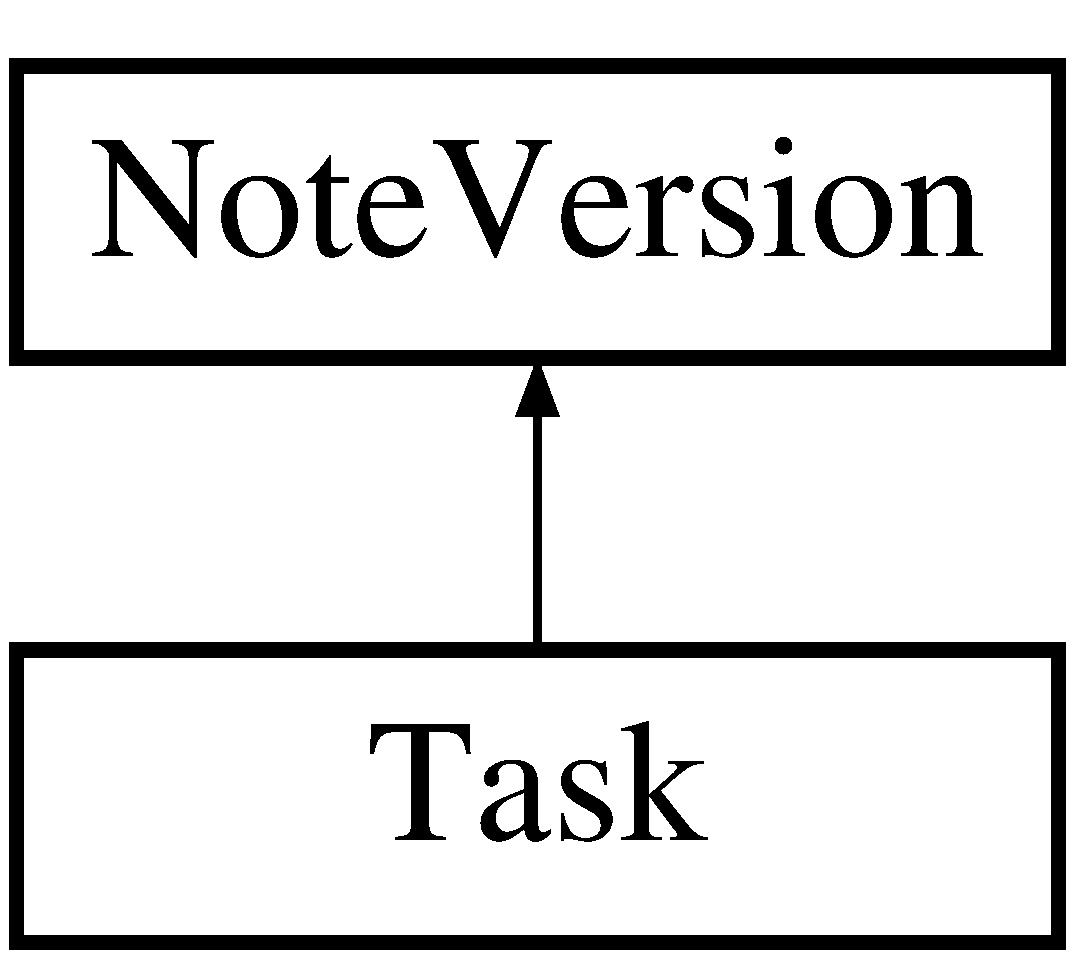
\includegraphics[height=2.000000cm]{class_task}
\end{center}
\end{figure}
\subsection*{Public Member Functions}
\begin{DoxyCompactItemize}
\item 
\hyperlink{class_task_a848131e6d6b7132cb77d636a3e2794c7}{Task} (const Q\+String \&t=Q\+String(), const Q\+String \&a=Q\+String(), unsigned int p=0, const \hyperlink{class_date}{Date} d=\hyperlink{class_date}{Date}(1, 1, 2100), const Status s=Status())
\begin{DoxyCompactList}\small\item\em Constructeur de la classe Tâche. \end{DoxyCompactList}\item 
\mbox{\Hypertarget{class_task_a90e80d51eae7ed6235497cd53a1f4930}\label{class_task_a90e80d51eae7ed6235497cd53a1f4930}} 
const Q\+String \& \hyperlink{class_task_a90e80d51eae7ed6235497cd53a1f4930}{get\+Action} () const
\begin{DoxyCompactList}\small\item\em accesseur pour obtenir l\textquotesingle{}action d\textquotesingle{}une tâche \end{DoxyCompactList}\item 
\mbox{\Hypertarget{class_task_a1f685a6b0201fd10d576e3b57ada937e}\label{class_task_a1f685a6b0201fd10d576e3b57ada937e}} 
unsigned int \hyperlink{class_task_a1f685a6b0201fd10d576e3b57ada937e}{get\+Priority} () const
\begin{DoxyCompactList}\small\item\em accesseur pour obtenir la prioritée d\textquotesingle{}une tâche \end{DoxyCompactList}\item 
\mbox{\Hypertarget{class_task_ab14cae63f329fae9a6db8257fb7b051c}\label{class_task_ab14cae63f329fae9a6db8257fb7b051c}} 
const \hyperlink{class_date}{Date} \& \hyperlink{class_task_ab14cae63f329fae9a6db8257fb7b051c}{get\+Deadline} () const
\begin{DoxyCompactList}\small\item\em accesseur pour obtenir la date deadline d\textquotesingle{}une tâche \end{DoxyCompactList}\item 
\mbox{\Hypertarget{class_task_a02289a96ff470980ee371f822e71f125}\label{class_task_a02289a96ff470980ee371f822e71f125}} 
const Status \& \hyperlink{class_task_a02289a96ff470980ee371f822e71f125}{get\+Status} () const
\begin{DoxyCompactList}\small\item\em accesseur pour obtenir le statut d\textquotesingle{}une tâche \end{DoxyCompactList}\item 
\hyperlink{class_task}{Task} $\ast$ \hyperlink{class_task_a1bbd4cedca0617ce64237e90af5a797a}{clone} (unsigned int id) const
\begin{DoxyCompactList}\small\item\em methode clone \end{DoxyCompactList}\item 
\mbox{\Hypertarget{class_task_ab7c7359a7703a41d4a46773443679213}\label{class_task_ab7c7359a7703a41d4a46773443679213}} 
Q\+String {\bfseries type} () const
\item 
\mbox{\Hypertarget{class_task_a9fd0d2efe3910eb438bbff7076a41d24}\label{class_task_a9fd0d2efe3910eb438bbff7076a41d24}} 
\hyperlink{class_form_version}{Form\+Version} $\ast$ {\bfseries form\+Version} ()
\end{DoxyCompactItemize}
\subsection*{Friends}
\begin{DoxyCompactItemize}
\item 
\mbox{\Hypertarget{class_task_a93d7e72623acdfa5b079a11fbf2d9f9d}\label{class_task_a93d7e72623acdfa5b079a11fbf2d9f9d}} 
class {\bfseries Note}
\end{DoxyCompactItemize}
\subsection*{Additional Inherited Members}


\subsection{Constructor \& Destructor Documentation}
\mbox{\Hypertarget{class_task_a848131e6d6b7132cb77d636a3e2794c7}\label{class_task_a848131e6d6b7132cb77d636a3e2794c7}} 
\index{Task@{Task}!Task@{Task}}
\index{Task@{Task}!Task@{Task}}
\subsubsection{\texorpdfstring{Task()}{Task()}}
{\footnotesize\ttfamily Task\+::\+Task (\begin{DoxyParamCaption}\item[{const Q\+String \&}]{t = {\ttfamily QString()},  }\item[{const Q\+String \&}]{a = {\ttfamily QString()},  }\item[{unsigned int}]{p = {\ttfamily 0},  }\item[{const \hyperlink{class_date}{Date}}]{d = {\ttfamily \hyperlink{class_date}{Date}(1,1,2100)},  }\item[{const Status}]{s = {\ttfamily Status()} }\end{DoxyParamCaption})}



Constructeur de la classe Tâche. 


\begin{DoxyParams}{Parameters}
{\em t} & titre de la tâche (utilisé par le constructeur de \hyperlink{class_note_version}{Note\+Version}) \\
\hline
{\em a} & action de la tâche \\
\hline
{\em p} & prioritée de la tâche \\
\hline
{\em d} & date de la tâche \\
\hline
{\em s} & statut de la tâche \\
\hline
\end{DoxyParams}


\subsection{Member Function Documentation}
\mbox{\Hypertarget{class_task_a1bbd4cedca0617ce64237e90af5a797a}\label{class_task_a1bbd4cedca0617ce64237e90af5a797a}} 
\index{Task@{Task}!clone@{clone}}
\index{clone@{clone}!Task@{Task}}
\subsubsection{\texorpdfstring{clone()}{clone()}}
{\footnotesize\ttfamily \hyperlink{class_task}{Task} $\ast$ Task\+::clone (\begin{DoxyParamCaption}\item[{unsigned int}]{id }\end{DoxyParamCaption}) const\hspace{0.3cm}{\ttfamily [virtual]}}



methode clone 

\begin{DoxyReturn}{Returns}
un pointeur de task sur le clone de la tâche grâce à l\textquotesingle{}id 
\end{DoxyReturn}

\begin{DoxyParams}{Parameters}
{\em id} & L\textquotesingle{}id de la tâche que l\textquotesingle{}on souhaite cloner \\
\hline
\end{DoxyParams}


Implements \hyperlink{class_note_version_a7eb23a52291ec623b9bc1b6fe3e86c5a}{Note\+Version}.



The documentation for this class was generated from the following files\+:\begin{DoxyCompactItemize}
\item 
Documents/\+U\+T\+C/\+G\+I02/\+L\+O21/\+L\+O21/\+Qt\+Version/\hyperlink{noteversion_8h}{noteversion.\+h}\item 
Documents/\+U\+T\+C/\+G\+I02/\+L\+O21/\+L\+O21/\+Qt\+Version/noteversion.\+cpp\end{DoxyCompactItemize}

\hypertarget{class_time_exception}{}\section{Time\+Exception Class Reference}
\label{class_time_exception}\index{Time\+Exception@{Time\+Exception}}
\subsection*{Public Member Functions}
\begin{DoxyCompactItemize}
\item 
\mbox{\Hypertarget{class_time_exception_a22a2308236c1b525d7910ac582c3a0c4}\label{class_time_exception_a22a2308236c1b525d7910ac582c3a0c4}} 
{\bfseries Time\+Exception} (const std\+::string \&m)
\item 
\mbox{\Hypertarget{class_time_exception_a4475d44829f2674ec87e2230e2424572}\label{class_time_exception_a4475d44829f2674ec87e2230e2424572}} 
const std\+::string \& {\bfseries Get\+Info} () const
\end{DoxyCompactItemize}


The documentation for this class was generated from the following file\+:\begin{DoxyCompactItemize}
\item 
Documents/\+G\+I02/\+L\+O21/\+Projet/\+L\+O21/\+Qt\+Version/\hyperlink{date_8h}{date.\+h}\end{DoxyCompactItemize}

\hypertarget{class_trash}{}\section{Trash Class Reference}
\label{class_trash}\index{Trash@{Trash}}
\subsection*{Public Member Functions}
\begin{DoxyCompactItemize}
\item 
\mbox{\Hypertarget{class_trash_a95c0683c6b1caebb3ab566a533a90876}\label{class_trash_a95c0683c6b1caebb3ab566a533a90876}} 
const std\+::vector$<$ \hyperlink{class_note}{Note} $\ast$ $>$ \& {\bfseries get\+List\+Trashed\+Notes} () const
\item 
\mbox{\Hypertarget{class_trash_ad2ae17877be5f9740176ee54f99704c7}\label{class_trash_ad2ae17877be5f9740176ee54f99704c7}} 
void \hyperlink{class_trash_ad2ae17877be5f9740176ee54f99704c7}{empty\+Trash} ()
\begin{DoxyCompactList}\small\item\em Fonction qui vide \hyperlink{class_trash}{Trash}. \end{DoxyCompactList}\item 
void \hyperlink{class_trash_a938c113450a14db9ff01d5747723f073}{add\+Note} (\hyperlink{class_note}{Note} $\ast$n)
\begin{DoxyCompactList}\small\item\em Fonction qui supprime une note de la \hyperlink{class_trash}{Trash}. \end{DoxyCompactList}\item 
void \hyperlink{class_trash_aab5b97637ce7706c0818261bfbdcbd05}{put\+Back\+Note} (unsigned int id)
\begin{DoxyCompactList}\small\item\em Fonction qui remet la note dans les notes actives (dans le tableau de notes de \hyperlink{class_notes_manager}{Notes\+Manager}) \end{DoxyCompactList}\item 
\mbox{\Hypertarget{class_trash_a65e68f34236ec1994a96292870ab8515}\label{class_trash_a65e68f34236ec1994a96292870ab8515}} 
void {\bfseries delete\+Note} (unsigned int id)
\end{DoxyCompactItemize}
\subsection*{Static Public Member Functions}
\begin{DoxyCompactItemize}
\item 
\mbox{\Hypertarget{class_trash_a7c07d5024656cf5770ab910482e717c9}\label{class_trash_a7c07d5024656cf5770ab910482e717c9}} 
static \hyperlink{class_trash}{Trash} \& \hyperlink{class_trash_a7c07d5024656cf5770ab910482e717c9}{get\+Instance} ()
\begin{DoxyCompactList}\small\item\em Fonction qui cree une instance de \hyperlink{class_trash}{Trash} s\textquotesingle{}il n\textquotesingle{}en existe pas une (\hyperlink{class_trash}{Trash} est une classe singleton) \end{DoxyCompactList}\item 
\mbox{\Hypertarget{class_trash_a45bcb2383f6114f7e5d3e2f3ad62e938}\label{class_trash_a45bcb2383f6114f7e5d3e2f3ad62e938}} 
static void \hyperlink{class_trash_a45bcb2383f6114f7e5d3e2f3ad62e938}{delete\+Instance} ()
\begin{DoxyCompactList}\small\item\em Fonction qui supprime une instance de \hyperlink{class_trash}{Trash} s\textquotesingle{}il en existe une. \end{DoxyCompactList}\end{DoxyCompactItemize}


\subsection{Member Function Documentation}
\mbox{\Hypertarget{class_trash_a938c113450a14db9ff01d5747723f073}\label{class_trash_a938c113450a14db9ff01d5747723f073}} 
\index{Trash@{Trash}!add\+Note@{add\+Note}}
\index{add\+Note@{add\+Note}!Trash@{Trash}}
\subsubsection{\texorpdfstring{add\+Note()}{addNote()}}
{\footnotesize\ttfamily void Trash\+::add\+Note (\begin{DoxyParamCaption}\item[{\hyperlink{class_note}{Note} $\ast$}]{n }\end{DoxyParamCaption})}



Fonction qui supprime une note de la \hyperlink{class_trash}{Trash}. 


\begin{DoxyParams}{Parameters}
{\em n} & note a retirer de la \hyperlink{class_trash}{Trash} \\
\hline
\end{DoxyParams}
\mbox{\Hypertarget{class_trash_aab5b97637ce7706c0818261bfbdcbd05}\label{class_trash_aab5b97637ce7706c0818261bfbdcbd05}} 
\index{Trash@{Trash}!put\+Back\+Note@{put\+Back\+Note}}
\index{put\+Back\+Note@{put\+Back\+Note}!Trash@{Trash}}
\subsubsection{\texorpdfstring{put\+Back\+Note()}{putBackNote()}}
{\footnotesize\ttfamily void Trash\+::put\+Back\+Note (\begin{DoxyParamCaption}\item[{unsigned int}]{id }\end{DoxyParamCaption})}



Fonction qui remet la note dans les notes actives (dans le tableau de notes de \hyperlink{class_notes_manager}{Notes\+Manager}) 


\begin{DoxyParams}{Parameters}
{\em n} & note a restaurer \\
\hline
\end{DoxyParams}


The documentation for this class was generated from the following files\+:\begin{DoxyCompactItemize}
\item 
Documents/\+U\+T\+C/\+G\+I02/\+L\+O21/\+L\+O21/\+Qt\+Version/trash.\+h\item 
Documents/\+U\+T\+C/\+G\+I02/\+L\+O21/\+L\+O21/\+Qt\+Version/trash.\+cpp\end{DoxyCompactItemize}

\hypertarget{class_trash_editor}{}\section{Trash\+Editor Class Reference}
\label{class_trash_editor}\index{Trash\+Editor@{Trash\+Editor}}
Inheritance diagram for Trash\+Editor\+:\begin{figure}[H]
\begin{center}
\leavevmode
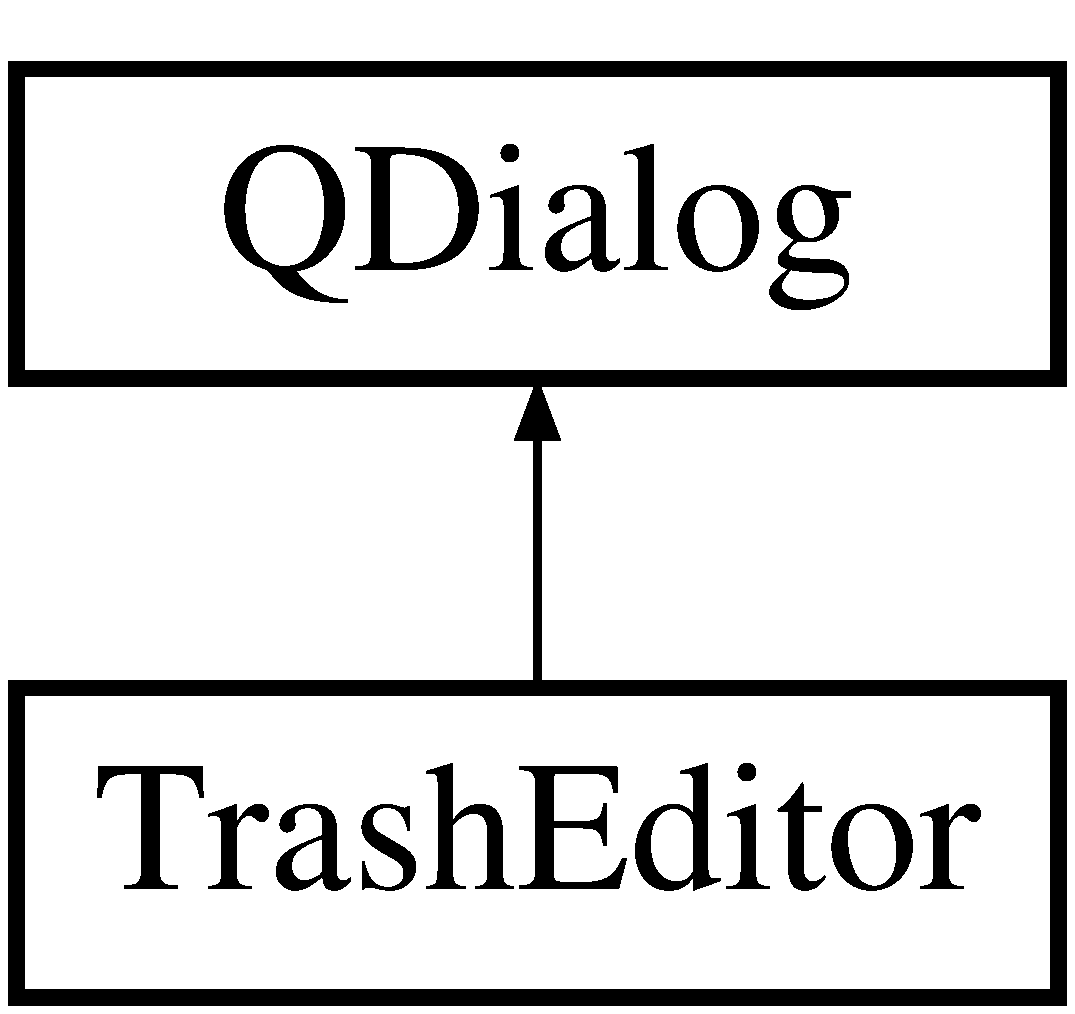
\includegraphics[height=2.000000cm]{class_trash_editor}
\end{center}
\end{figure}
\subsection*{Public Member Functions}
\begin{DoxyCompactItemize}
\item 
\mbox{\Hypertarget{class_trash_editor_a7a106bef91b37afbc201c7742986bdb5}\label{class_trash_editor_a7a106bef91b37afbc201c7742986bdb5}} 
{\bfseries Trash\+Editor} (Q\+Widget $\ast$parent=0)
\item 
\mbox{\Hypertarget{class_trash_editor_adebdb1b69887257d460f66e3de2ae24a}\label{class_trash_editor_adebdb1b69887257d460f66e3de2ae24a}} 
void {\bfseries load\+Trashed\+Notes} ()
\end{DoxyCompactItemize}


The documentation for this class was generated from the following files\+:\begin{DoxyCompactItemize}
\item 
Documents/\+U\+T\+C/\+G\+I02/\+L\+O21/\+L\+O21/\+Qt\+Version/trasheditor.\+h\item 
Documents/\+U\+T\+C/\+G\+I02/\+L\+O21/\+L\+O21/\+Qt\+Version/trasheditor.\+cpp\end{DoxyCompactItemize}

\hypertarget{classtype_note}{}\section{type\+Note Class Reference}
\label{classtype_note}\index{type\+Note@{type\+Note}}
Inheritance diagram for type\+Note\+:\begin{figure}[H]
\begin{center}
\leavevmode
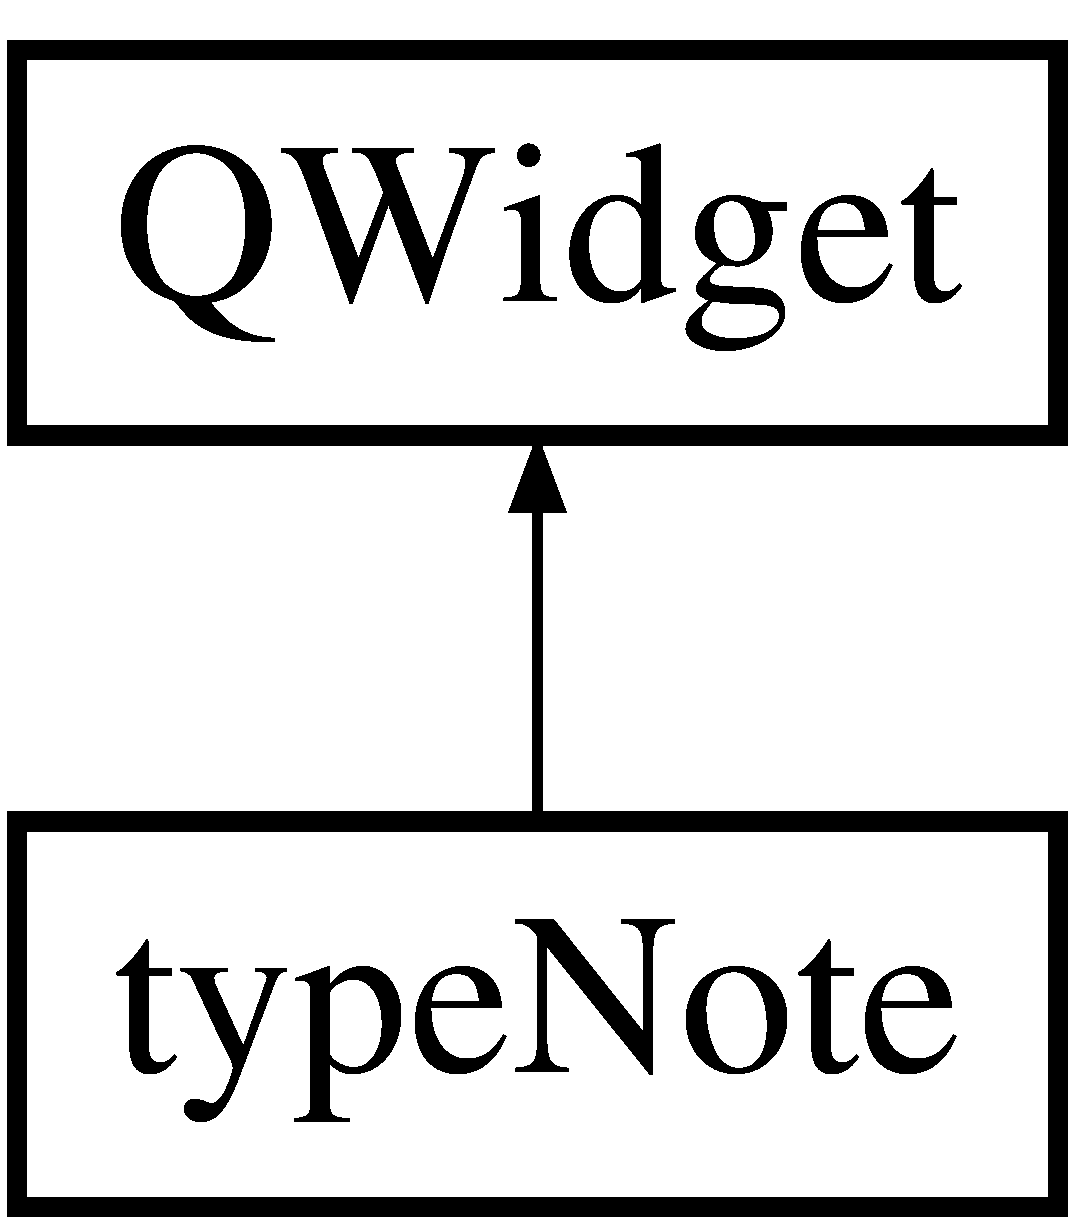
\includegraphics[height=2.000000cm]{classtype_note}
\end{center}
\end{figure}
\subsection*{Public Member Functions}
\begin{DoxyCompactItemize}
\item 
\mbox{\Hypertarget{classtype_note_a9e9ce5085521858a5b36d76d66618c2b}\label{classtype_note_a9e9ce5085521858a5b36d76d66618c2b}} 
{\bfseries type\+Note} (\hyperlink{class_notes_manager}{Notes\+Manager} $\ast$m, Q\+Widget $\ast$parent=0)
\item 
\mbox{\Hypertarget{classtype_note_a367f23d98b0f1d749a6f4ee18998bf38}\label{classtype_note_a367f23d98b0f1d749a6f4ee18998bf38}} 
void {\bfseries load\+Types} ()
\item 
\mbox{\Hypertarget{classtype_note_a1ab64b02b765f812ab4ab8a9e527865e}\label{classtype_note_a1ab64b02b765f812ab4ab8a9e527865e}} 
void {\bfseries on\+\_\+validate\+\_\+clicked} ()
\end{DoxyCompactItemize}


The documentation for this class was generated from the following files\+:\begin{DoxyCompactItemize}
\item 
Documents/\+U\+T\+C/\+G\+I02/\+L\+O21/\+L\+O21/\+Qt\+Version/mainwindow.\+h\item 
Documents/\+U\+T\+C/\+G\+I02/\+L\+O21/\+L\+O21/\+Qt\+Version/mainwindow.\+cpp\end{DoxyCompactItemize}

\hypertarget{class_video}{}\section{Video Class Reference}
\label{class_video}\index{Video@{Video}}
Inheritance diagram for Video\+:\begin{figure}[H]
\begin{center}
\leavevmode
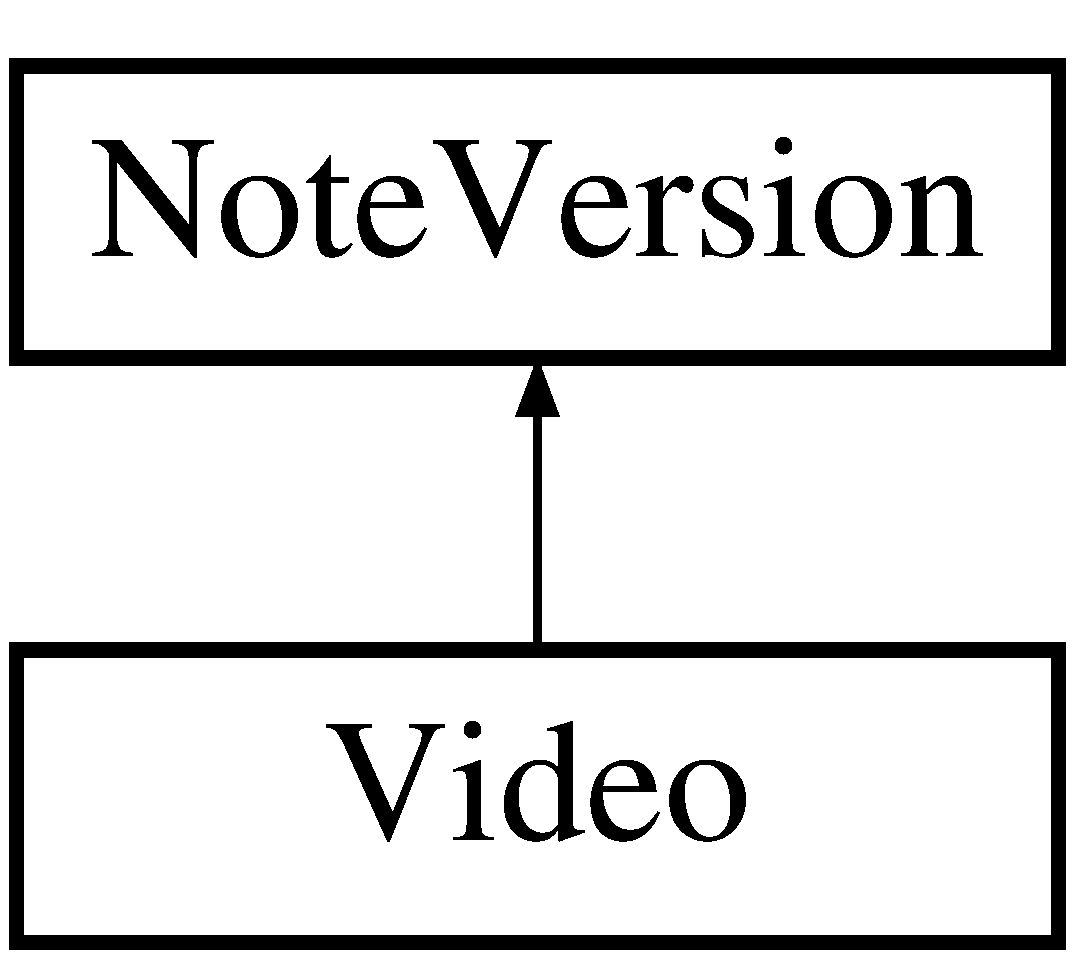
\includegraphics[height=2.000000cm]{class_video}
\end{center}
\end{figure}
\subsection*{Public Member Functions}
\begin{DoxyCompactItemize}
\item 
\hyperlink{class_video_a4a902371a9cf3d9d2c6300f181745646}{Video} (const Q\+String \&t, const Q\+String \&d, const Q\+String \&f)
\begin{DoxyCompactList}\small\item\em Constructeur de la classe \hyperlink{class_video}{Video}. \end{DoxyCompactList}\item 
\mbox{\Hypertarget{class_video_a7f921dc22bb8b7c4fd6551cd6d61a957}\label{class_video_a7f921dc22bb8b7c4fd6551cd6d61a957}} 
const Q\+String \& \hyperlink{class_video_a7f921dc22bb8b7c4fd6551cd6d61a957}{get\+Description} () const
\begin{DoxyCompactList}\small\item\em accesseur pour obtenir la description d\textquotesingle{}une note \hyperlink{class_video}{Video} \end{DoxyCompactList}\item 
\mbox{\Hypertarget{class_video_af2019c98a6abc6bd6334137155c9b06d}\label{class_video_af2019c98a6abc6bd6334137155c9b06d}} 
const Q\+String \& \hyperlink{class_video_af2019c98a6abc6bd6334137155c9b06d}{get\+File} () const
\begin{DoxyCompactList}\small\item\em accesseur pour obtenir le fichier d\textquotesingle{}une note \hyperlink{class_video}{Video} \end{DoxyCompactList}\item 
\hyperlink{class_video}{Video} $\ast$ \hyperlink{class_video_a505ceb0063f73cf8dd06bc6c6ff72c5d}{clone} (unsigned int id) const
\begin{DoxyCompactList}\small\item\em methode clone \end{DoxyCompactList}\item 
\mbox{\Hypertarget{class_video_a0fa52bee53c7b9c860cf4a9db34ea512}\label{class_video_a0fa52bee53c7b9c860cf4a9db34ea512}} 
Q\+String {\bfseries type} () const
\item 
\mbox{\Hypertarget{class_video_a8ee5b9f6239ba930dd6445e01100336f}\label{class_video_a8ee5b9f6239ba930dd6445e01100336f}} 
\hyperlink{class_form_version}{Form\+Version} $\ast$ {\bfseries form\+Version} ()
\end{DoxyCompactItemize}
\subsection*{Friends}
\begin{DoxyCompactItemize}
\item 
\mbox{\Hypertarget{class_video_a93d7e72623acdfa5b079a11fbf2d9f9d}\label{class_video_a93d7e72623acdfa5b079a11fbf2d9f9d}} 
class {\bfseries Note}
\end{DoxyCompactItemize}
\subsection*{Additional Inherited Members}


\subsection{Constructor \& Destructor Documentation}
\mbox{\Hypertarget{class_video_a4a902371a9cf3d9d2c6300f181745646}\label{class_video_a4a902371a9cf3d9d2c6300f181745646}} 
\index{Video@{Video}!Video@{Video}}
\index{Video@{Video}!Video@{Video}}
\subsubsection{\texorpdfstring{Video()}{Video()}}
{\footnotesize\ttfamily Video\+::\+Video (\begin{DoxyParamCaption}\item[{const Q\+String \&}]{t,  }\item[{const Q\+String \&}]{d,  }\item[{const Q\+String \&}]{f }\end{DoxyParamCaption})}



Constructeur de la classe \hyperlink{class_video}{Video}. 


\begin{DoxyParams}{Parameters}
{\em t} & titre d\textquotesingle{}une note \hyperlink{class_video}{Video} (utilisé par le constructeur de \hyperlink{class_note_version}{Note\+Version}) \\
\hline
{\em d} & description d\textquotesingle{}une note \hyperlink{class_video}{Video} \\
\hline
{\em f} & fichier d\textquotesingle{}une note video \\
\hline
\end{DoxyParams}


\subsection{Member Function Documentation}
\mbox{\Hypertarget{class_video_a505ceb0063f73cf8dd06bc6c6ff72c5d}\label{class_video_a505ceb0063f73cf8dd06bc6c6ff72c5d}} 
\index{Video@{Video}!clone@{clone}}
\index{clone@{clone}!Video@{Video}}
\subsubsection{\texorpdfstring{clone()}{clone()}}
{\footnotesize\ttfamily \hyperlink{class_video}{Video} $\ast$ Video\+::clone (\begin{DoxyParamCaption}\item[{unsigned int}]{id }\end{DoxyParamCaption}) const\hspace{0.3cm}{\ttfamily [virtual]}}



methode clone 

\begin{DoxyReturn}{Returns}
un pointeur de \hyperlink{class_video}{Video} sur le clone de la note \hyperlink{class_video}{Video} grâce à l\textquotesingle{}id 
\end{DoxyReturn}

\begin{DoxyParams}{Parameters}
{\em id} & L\textquotesingle{}id de la note \hyperlink{class_video}{Video} que l\textquotesingle{}on souhaite cloner \\
\hline
\end{DoxyParams}


Implements \hyperlink{class_note_version_a7eb23a52291ec623b9bc1b6fe3e86c5a}{Note\+Version}.



The documentation for this class was generated from the following files\+:\begin{DoxyCompactItemize}
\item 
Documents/\+G\+I02/\+L\+O21/\+Projet/\+L\+O21/\+Qt\+Version/\hyperlink{noteversion_8h}{noteversion.\+h}\item 
Documents/\+G\+I02/\+L\+O21/\+Projet/\+L\+O21/\+Qt\+Version/noteversion.\+cpp\end{DoxyCompactItemize}

\chapter{File Documentation}
\hypertarget{date_8h}{}\section{Documents/\+G\+I02/\+L\+O21/\+Projet/\+L\+O21/\+Qt\+Version/date.h File Reference}
\label{date_8h}\index{Documents/\+G\+I02/\+L\+O21/\+Projet/\+L\+O21/\+Qt\+Version/date.\+h@{Documents/\+G\+I02/\+L\+O21/\+Projet/\+L\+O21/\+Qt\+Version/date.\+h}}


Définition du type date.  


{\ttfamily \#include $<$iostream$>$}\newline
{\ttfamily \#include $<$iomanip$>$}\newline
\subsection*{Classes}
\begin{DoxyCompactItemize}
\item 
class \hyperlink{class_time_exception}{Time\+Exception}
\item 
class \hyperlink{class_date}{Date}
\end{DoxyCompactItemize}


\subsection{Detailed Description}
Définition du type date. 

Nous avons définit le type date afin de pouvoir l\textquotesingle{}utiliser dans nos différentes fonctions de classes plus tard 
\hypertarget{note_8h}{}\section{Documents/\+G\+I02/\+L\+O21/\+Projet/\+L\+O21/\+Qt\+Version/note.h File Reference}
\label{note_8h}\index{Documents/\+G\+I02/\+L\+O21/\+Projet/\+L\+O21/\+Qt\+Version/note.\+h@{Documents/\+G\+I02/\+L\+O21/\+Projet/\+L\+O21/\+Qt\+Version/note.\+h}}


Définition de la classe \hyperlink{class_note}{Note}.  


{\ttfamily \#include \char`\"{}noteversion.\+h\char`\"{}}\newline
{\ttfamily \#include $<$Q\+Xml\+Stream\+Writer$>$}\newline
\subsection*{Classes}
\begin{DoxyCompactItemize}
\item 
class \hyperlink{class_note}{Note}
\item 
class \hyperlink{class_exception}{Exception}
\end{DoxyCompactItemize}
\subsection*{Enumerations}
\begin{DoxyCompactItemize}
\item 
enum \hyperlink{note_8h_adc6e5733fc3c22f0a7b2914188c49c90}{state} \{ {\bfseries active} =1, 
{\bfseries archived} =0, 
{\bfseries trashed} =-\/1
 \}\begin{DoxyCompactList}\small\item\em création du type state \end{DoxyCompactList}
\end{DoxyCompactItemize}


\subsection{Detailed Description}
Définition de la classe \hyperlink{class_note}{Note}. 

La classe note est une amie de la classe \hyperlink{class_notes_manager}{Notes\+Manager}, on y définit les différents attributs et méthodes qui caractérise une notes en général. 

\subsection{Enumeration Type Documentation}
\mbox{\Hypertarget{note_8h_adc6e5733fc3c22f0a7b2914188c49c90}\label{note_8h_adc6e5733fc3c22f0a7b2914188c49c90}} 
\index{note.\+h@{note.\+h}!state@{state}}
\index{state@{state}!note.\+h@{note.\+h}}
\subsubsection{\texorpdfstring{state}{state}}
{\footnotesize\ttfamily enum \hyperlink{note_8h_adc6e5733fc3c22f0a7b2914188c49c90}{state}}



création du type state 

Nous avons créer une enumération state afin de définir l\textquotesingle{}état d\textquotesingle{}une note, 1 -\/$>$ la note est active, 0 -\/$>$ la note est supprimée par l\textquotesingle{}utilisateur mais comme elle est en relation avec une autre elle est dans un état archivée, -\/1 -\/$>$ la note est dans la corbeille en attendant d\textquotesingle{}être supprimée définitivement lorsque la corbeille sera vidée. 
\hypertarget{notesmanager_8h}{}\section{Documents/\+U\+T\+C/\+G\+I02/\+L\+O21/\+L\+O21/\+Qt\+Version/notesmanager.h File Reference}
\label{notesmanager_8h}\index{Documents/\+U\+T\+C/\+G\+I02/\+L\+O21/\+L\+O21/\+Qt\+Version/notesmanager.\+h@{Documents/\+U\+T\+C/\+G\+I02/\+L\+O21/\+L\+O21/\+Qt\+Version/notesmanager.\+h}}


Définition de la classe \hyperlink{class_notes_manager}{Notes\+Manager}.  


{\ttfamily \#include \char`\"{}note.\+h\char`\"{}}\newline
{\ttfamily \#include \char`\"{}trash.\+h\char`\"{}}\newline
\subsection*{Classes}
\begin{DoxyCompactItemize}
\item 
class \hyperlink{class_notes_manager}{Notes\+Manager}
\end{DoxyCompactItemize}


\subsection{Detailed Description}
Définition de la classe \hyperlink{class_notes_manager}{Notes\+Manager}. 

La classe \hyperlink{class_notes_manager}{Notes\+Manager}, on y définit les différents attributs et méthodes qui caractérise la gestion des notes au sein de l\textquotesingle{}application pluri\+Notes.

La relation entre les classes \hyperlink{class_notes_manager}{Notes\+Manager} et \hyperlink{class_note}{Note} est une composition 
\hypertarget{noteversion_8h}{}\section{Documents/\+G\+I02/\+L\+O21/\+Projet/\+L\+O21/\+Qt\+Version/noteversion.h File Reference}
\label{noteversion_8h}\index{Documents/\+G\+I02/\+L\+O21/\+Projet/\+L\+O21/\+Qt\+Version/noteversion.\+h@{Documents/\+G\+I02/\+L\+O21/\+Projet/\+L\+O21/\+Qt\+Version/noteversion.\+h}}


Définition de la classe \hyperlink{class_note_version}{Note\+Version}.  


{\ttfamily \#include $<$iostream$>$}\newline
{\ttfamily \#include $<$Q\+Application$>$}\newline
{\ttfamily \#include $<$Q\+String$>$}\newline
{\ttfamily \#include $<$Q\+File\+Dialog$>$}\newline
{\ttfamily \#include $<$vector$>$}\newline
{\ttfamily \#include $<$Q\+Debug$>$}\newline
{\ttfamily \#include \char`\"{}date.\+h\char`\"{}}\newline
{\ttfamily \#include $<$Q\+H\+Box\+Layout$>$}\newline
{\ttfamily \#include $<$Q\+Label$>$}\newline
{\ttfamily \#include $<$Q\+Main\+Window$>$}\newline
{\ttfamily \#include $<$Q\+Object$>$}\newline
{\ttfamily \#include $<$Q\+Text\+Edit$>$}\newline
{\ttfamily \#include $<$Q\+Widget$>$}\newline
{\ttfamily \#include $<$Q\+Xml\+Stream\+Writer$>$}\newline
\subsection*{Classes}
\begin{DoxyCompactItemize}
\item 
class \hyperlink{class_note_version}{Note\+Version}
\item 
class \hyperlink{class_note_version_factory}{Note\+Version\+Factory}
\item 
struct \hyperlink{struct_derived_register}{Derived\+Register$<$ T $>$}
\item 
class \hyperlink{class_article}{Article}
\item 
class \hyperlink{class_task}{Task}
\item 
class \hyperlink{class_image}{Image}
\item 
class \hyperlink{class_audio}{Audio}
\item 
class \hyperlink{class_video}{Video}
\item 
class \hyperlink{class_form_version}{Form\+Version}
\item 
class \hyperlink{class_form_article}{Form\+Article}
\item 
class \hyperlink{class_form_image}{Form\+Image}
\end{DoxyCompactItemize}
\subsection*{Functions}
\begin{DoxyCompactItemize}
\item 
\mbox{\Hypertarget{noteversion_8h_ac7659cf68afdf606c75affe7d277fc32}\label{noteversion_8h_ac7659cf68afdf606c75affe7d277fc32}} 
{\footnotesize template$<$typename T $>$ }\\\hyperlink{class_note_version}{Note\+Version} $\ast$ \hyperlink{noteversion_8h_ac7659cf68afdf606c75affe7d277fc32}{createT} ()
\begin{DoxyCompactList}\small\item\em Utilisée pour les méthodes de chargement. \end{DoxyCompactList}\end{DoxyCompactItemize}


\subsection{Detailed Description}
Définition de la classe \hyperlink{class_note_version}{Note\+Version}. 

La classe \hyperlink{class_note_version}{Note\+Version} est une amie de la classe \hyperlink{class_note}{Note}, une version de note peut être un article, un fichier image, un fichier vidéo, un fichier son ou une tâche. 
\hypertarget{plurinotes_8h}{}\section{Documents/\+U\+T\+C/\+G\+I02/\+L\+O21/\+L\+O21/\+Qt\+Version/plurinotes.h File Reference}
\label{plurinotes_8h}\index{Documents/\+U\+T\+C/\+G\+I02/\+L\+O21/\+L\+O21/\+Qt\+Version/plurinotes.\+h@{Documents/\+U\+T\+C/\+G\+I02/\+L\+O21/\+L\+O21/\+Qt\+Version/plurinotes.\+h}}
{\ttfamily \#include $<$iostream$>$}\newline
{\ttfamily \#include $<$Q\+Application$>$}\newline
{\ttfamily \#include $<$Q\+String$>$}\newline
{\ttfamily \#include $<$Q\+File\+Dialog$>$}\newline
{\ttfamily \#include $<$vector$>$}\newline
{\ttfamily \#include \char`\"{}date.\+h\char`\"{}}\newline

\hypertarget{relation_8h}{}\section{Documents/\+G\+I02/\+L\+O21/\+Projet/\+L\+O21/\+Qt\+Version/relation.h File Reference}
\label{relation_8h}\index{Documents/\+G\+I02/\+L\+O21/\+Projet/\+L\+O21/\+Qt\+Version/relation.\+h@{Documents/\+G\+I02/\+L\+O21/\+Projet/\+L\+O21/\+Qt\+Version/relation.\+h}}


Définition de la classe \hyperlink{class_couple}{Couple} et \hyperlink{class_relation}{Relation}.  


{\ttfamily \#include \char`\"{}note.\+h\char`\"{}}\newline
\subsection*{Classes}
\begin{DoxyCompactItemize}
\item 
class \hyperlink{class_couple}{Couple}
\item 
class \hyperlink{class_relation}{Relation}
\end{DoxyCompactItemize}


\subsection{Detailed Description}
Définition de la classe \hyperlink{class_couple}{Couple} et \hyperlink{class_relation}{Relation}. 

La classe \hyperlink{class_couple}{Couple} définit les caractéristiques d\textquotesingle{}un couple de notes dans une relation.

La classe \hyperlink{class_relation}{Relation} définit les attributs et les méthodes des relations. 
%--- End generated contents ---

% Index
\backmatter
\newpage
\phantomsection
\clearemptydoublepage
\addcontentsline{toc}{chapter}{Index}
\printindex

\end{document}
